%% ============================================================
%%  Beamer slides — Extension v5 (CSP styled)
%%  Supervisor discussion deck, v1..v5 tracking
%%  Compile: pdflatex extension_v5_slides_csp.tex (twice)
%% ============================================================
\documentclass[10pt,aspectratio=169]{beamer}

% ---- CSP style ---------------------------------------------------------
\usepackage{CSPstyles}

% ---- theme: minimal default + CSP palette ------------------------------
\usetheme{default}
\useinnertheme{rectangles}
\setbeamertemplate{navigation symbols}{}
\setbeamertemplate{footline}[frame number]
\setbeamercolor{structure}{fg=CSP-main-dark}
\setbeamercolor{frametitle}{fg=CSP-main-dark}
\setbeamercolor{title}{fg=CSP-main-dark}
\setbeamercolor{subtitle}{fg=CSP-text}
\setbeamercolor{author}{fg=CSP-text}
\setbeamercolor{date}{fg=CSP-text-light}
\setbeamercolor{itemize item}{fg=CSP-main}
\setbeamercolor{itemize subitem}{fg=CSP-main-light}
\setbeamercolor{alerted text}{fg=CSP-emphasis}
\setbeamercolor{normal text}{fg=CSP-text}
\setbeamercolor{block title}{bg=CSP-main-light, fg=CSP-text-dark}
\setbeamercolor{block body}{bg=independence-light-5, fg=CSP-text}
\setbeamerfont{frametitle}{series=\bfseries}
\setbeamerfont{title}{series=\bfseries,size=\LARGE}

% ---- packages ----------------------------------------------------------
\usepackage{booktabs}
\usepackage{array}
\usepackage{graphicx}
\graphicspath{{../../05-modelling-production-data/figures/v5/}{../../05-modelling-production-data/figures/}{../figures/}}
\usepackage{amsmath, amssymb, bm}
\usepackage{colortbl}

% convenience macros (on top of CSPstyles' \emphasis, \accentone, ...)
\newcommand{\main}[1]{\textcolor{CSP-main-dark}{\textbf{#1}}}
\newcommand{\emp}[1]{\textcolor{CSP-emphasis}{\textbf{#1}}}
\newcommand{\acct}[1]{\textcolor{CSP-accent-1-dark}{#1}}      % teal accent
\newcommand{\accy}[1]{\textcolor{CSP-accent-2-dark}{#1}}      % orange/gold
\newcommand{\accg}[1]{\textcolor{CSP-accent-3-dark}{#1}}      % green
\newcommand{\muted}[1]{\textcolor{CSP-text-light}{#1}}

\title{RSAop - Exploration of Production Model Extensions}
\date{2026-04-20}

\begin{document}

% ====================================================================
\begin{frame}
\titlepage
\end{frame}

% ====================================================================
\begin{frame}{Where we start: the paper-reported model}
\small
A $2\!\times\!2$ comparison: speaker architecture $\times$ semantics regime.

\vspace{0.3em}
\begin{itemize}\itemsep0.15em
  \item Architecture --- \emph{incremental}: utterances are built word-by-word, updating the literal listener after each word; \emph{global}: entire utterances are scored at once.
  \item Semantics --- \emph{recursive}: adjective thresholds adapt to the listener's running posterior at each step; \emph{static}: thresholds fixed from the uniform prior.
\end{itemize}

\vspace{0.3em}
Beyond the $2\!\times\!2$, the model has a single rationality $\alpha$ (shared across dimensions), an LM prior weighted by $\beta = \exp(\log\beta)$, and hierarchical per-participant offsets $\delta_p$ on $\alpha$.
Length bias $\gamma = 0$ and lapse $\varepsilon = 0$ are fixed.

\vspace{0.3em}
$2\!\times\!2$ result:
\begin{center}\footnotesize
\begin{tabular}{lrrrrr}
\toprule
Model & ELPD LOO & $\Delta$ ELPD & dSE & $\Delta$/dSE & $p$\\
\midrule
\main{Inc.\ context-updating} & \main{$-6985$} & $0$ & --- & --- & ---\\
Inc.\ context-fixed           & $-7001$ & $-15.6$  & 1.5  & $-10.4$ & $<.001$\\
Global context-updating       & $-7728$ & $-742.8$ & 45.0 & $-16.5$ & $<.001$\\
Global context-fixed          & $-7739$ & $-753.2$ & 44.8 & $-16.8$ & $<.001$\\
\bottomrule
\end{tabular}
\end{center}

\vspace{0.2em}
\begin{itemize}\itemsep0.15em
  \item Architecture effect is large: incremental $\gg$ global ($\Delta/$dSE $\approx 16.5$).
  \item Within incremental, context-updating helps ($\Delta/$dSE $= 10.4$); within global, the two regimes are effectively tied ($\Delta\text{ELPD} \approx 10$).
\end{itemize}
\end{frame}

% ====================================================================
\begin{frame}{The data fit is nevertheless not optimal}
\small
\begin{itemize}\itemsep0.3em
  \item $R^2 = 0.41$ across the 90 (condition $\times$ utterance) cells.
  \item Neither lapse nor length bias is in the reported model: $\gamma$ and $\varepsilon$ are hardcoded to $0$, so all mass comes from the RSA softmax.
\end{itemize}

\vspace{0.5em}
Seven meaningful residuals that worth diagnosing and fixing:
\begin{center}\footnotesize
\begin{tabular}{lll rrr}
\toprule
Condition & Sharpness & Utterance & Emp & Model & $\Delta$\\
\midrule
colour-sufficient & high & C   & .716 & .352 & $\emp{-.364}$\\
colour-sufficient & low  & C   & .628 & .341 & $\emp{-.287}$\\
size-sufficient   & low  & D   & .056 & .324 & $\emp{+.268}$\\
size-sufficient   & low  & DCF & .300 & .068 & $\emp{-.233}$\\
both-necessary    & low  & CF  & .270 & .057 & $\emp{-.213}$\\
both-necessary    & high & D   & .000 & .206 & $\emp{+.206}$\\
both-necessary    & low  & DCF & .310 & .109 & $\emp{-.201}$\\
\bottomrule
\end{tabular}
\end{center}
\end{frame}

% ====================================================================
\begin{frame}{Paper-reported model: posterior predictive check}
\vspace{-0.3em}
\begin{center}
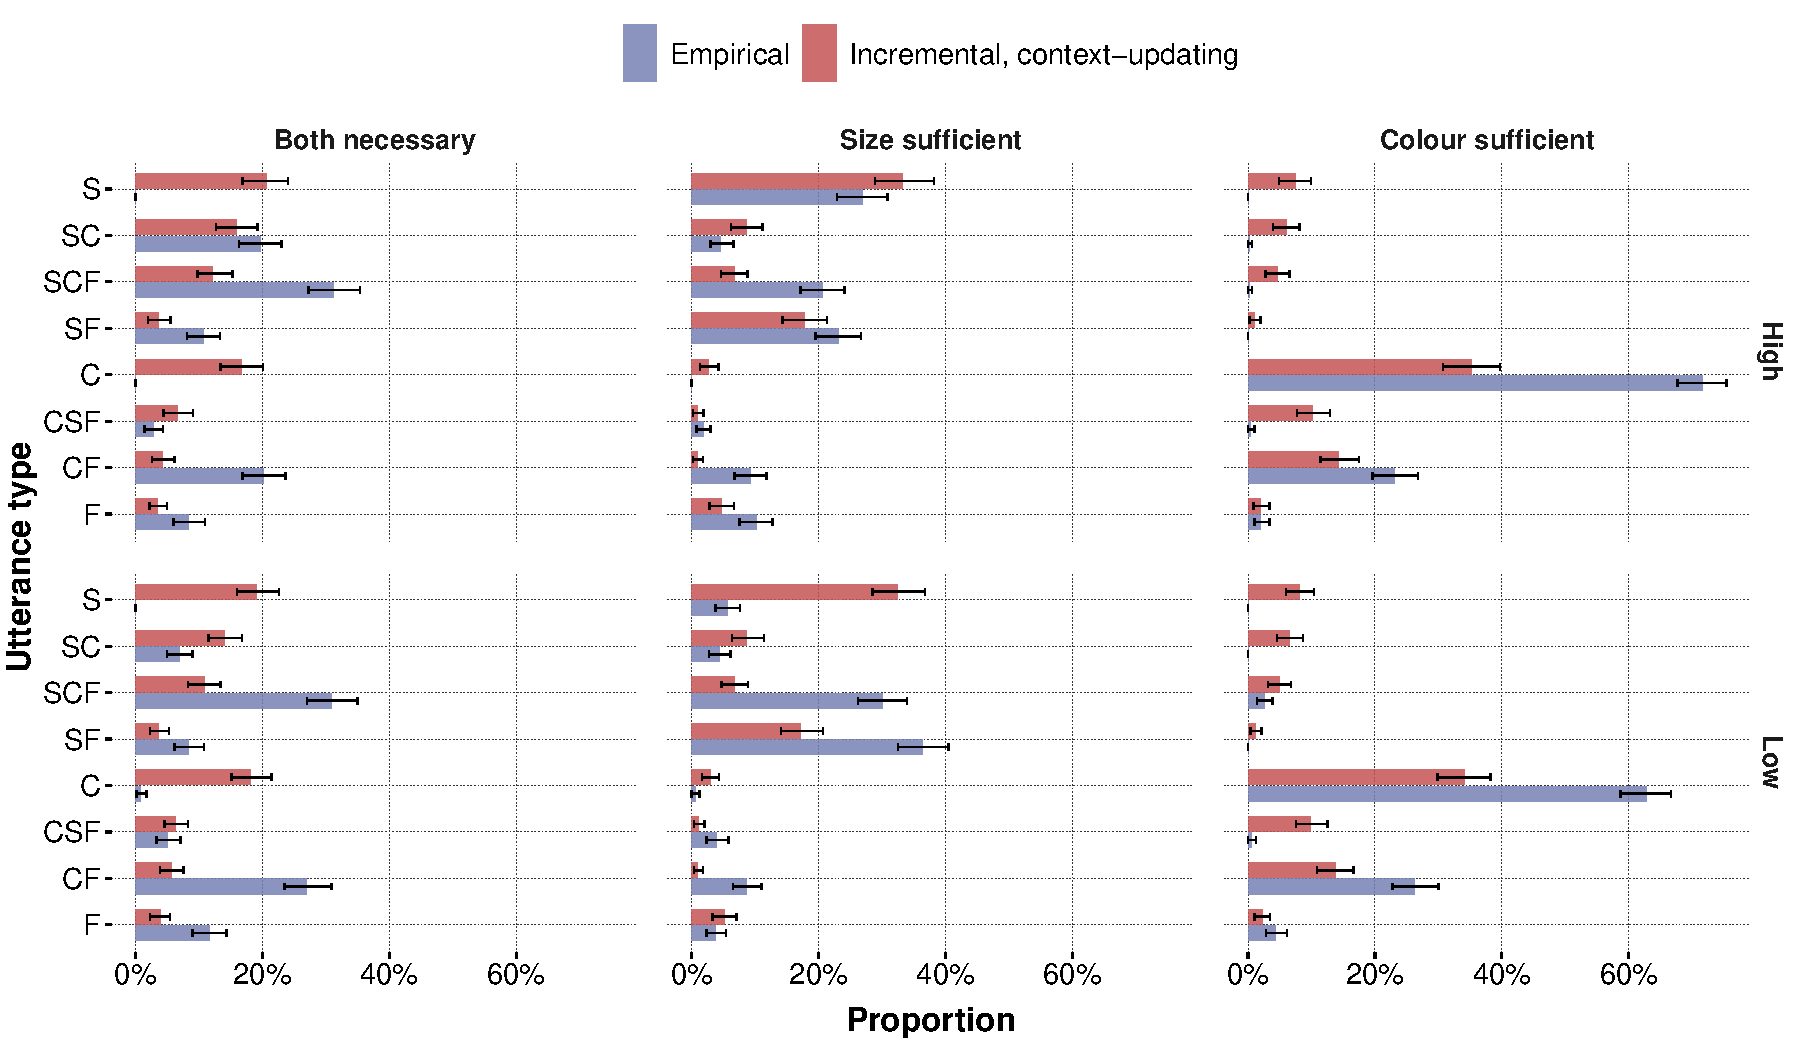
\includegraphics[width=0.82\linewidth]{production_ppc_barplot.pdf}
\end{center}
\vspace{0.2em}
\footnotesize
Empirical (blue) vs predicted (red) utterance proportions by condition $\times$ sharpness. Model mass is spread too evenly: colour-sufficient C is under-predicted and both-necessary C over-predicted.
\end{frame}

% ====================================================================
\begin{frame}{Paper-reported model: predicted vs observed}
\vspace{-0.3em}
\begin{center}
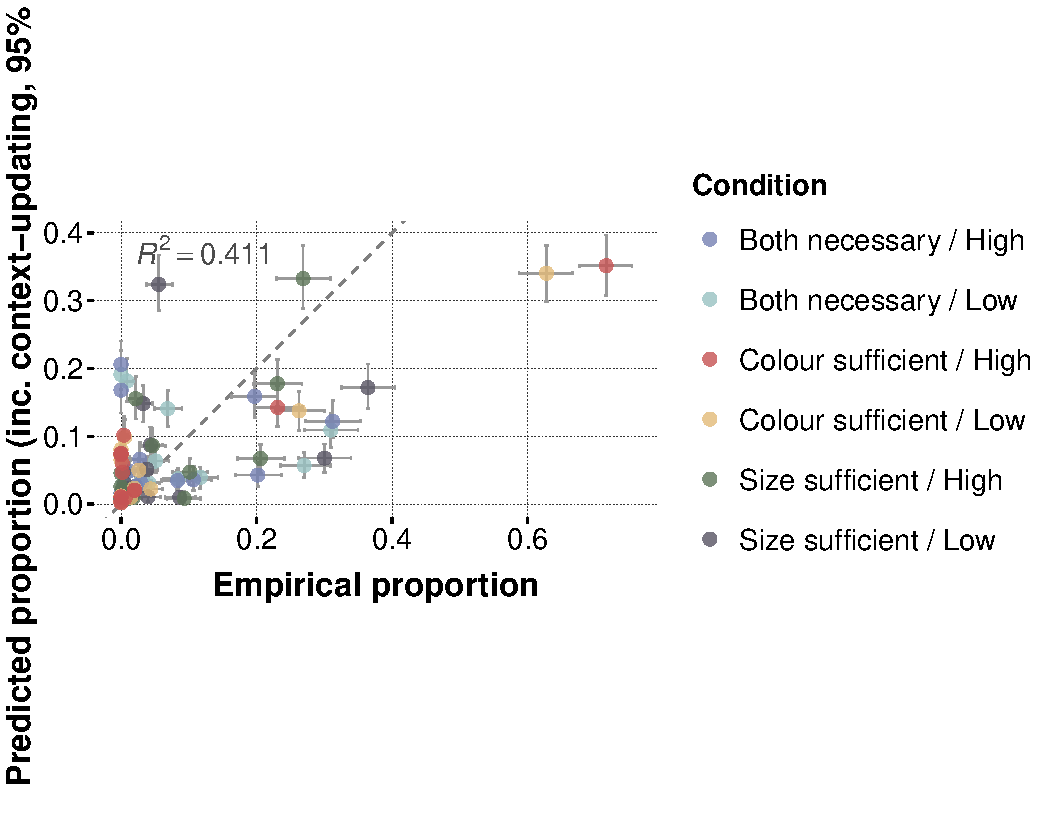
\includegraphics[width=0.58\linewidth]{production_correlation_inc_hier.pdf}
\end{center}
\vspace{0.2em}
\footnotesize
Predicted vs observed across all 90 condition $\times$ utterance cells; $R^2 = .41$.
\end{frame}

% ====================================================================
\begin{frame}{Diagnosis}
\small
The seven residuals decompose along two largely independent axes.

\vspace{0.5em}
\main{1.~Bare C is under-predicted when colour is sufficient}
\begin{itemize}\itemsep0.1em
  \item high sharpness: $.716 \to .352$ ($\Delta = -.36$); low: $.628 \to .341$ ($\Delta = -.29$).
  \item A single $\alpha$ cannot concentrate enough mass on C in this context; the model spreads probability across C-initial compounds.
  \item Points to a condition-gated colour boost ($\lambda_C$ in v5a).
\end{itemize}

\vspace{0.5em}
\main{2.~Length structure: bare D over-predicted, multi-adjective utterances under-predicted}
\begin{itemize}\itemsep0.1em
  \item bare D: size-sufficient / low $.056 \to .324$ ($+.27$); both-necessary / high $.000 \to .206$ ($+.21$).
  \item CF: both-necessary / low $.270 \to .057$ ($-.21$).
  \item DCF: size-sufficient / low $.300 \to .068$ ($-.23$); both-necessary / low $.310 \to .109$ ($-.20$).
  \item With $\gamma = 0$ in the reported model there is no utility boost for longer utterances, so the model defaults to the shortest informative form. Over-specification is also larger under blur and asymmetric across conditions, so no monotone linear $\gamma$ fits all three.
  \item Points to an explicit length bias ($\gamma$, $\gamma_1, \gamma_2$) plus condition- ($\delta\gamma$) and sharpness-dependent ($\eta$) offsets.
\end{itemize}

\vspace{0.4em}
These two diagnostics motivate the mechanism track below.
\end{frame}

% ====================================================================
\begin{frame}{Why these diagnostics are hard to fix jointly}
\small
\main{A single $\alpha$ cannot concentrate and spread at once.}
\begin{itemize}\itemsep0.1em
  \item Axis 1 wants near-degenerate mass on bare C; axis 2 wants mass spread across multi-adjective forms.
  \item Raising $\alpha$ concentrates everywhere, lowering it spreads everywhere --- a single $\alpha$ lands at a compromise.
\end{itemize}

\vspace{0.5em}
\main{A single linear $\gamma$ cannot be selectively positive.}
\begin{itemize}\itemsep0.1em
  \item Axis 2 wants a length boost in both-necessary and blurred size-sufficient --- but not in colour-sufficient, and smaller under high sharpness.
  \item Any $\gamma$ large enough to recover DCF in size-sufficient also inflates multi-adjective forms in colour-sufficient. v5b confirms: no condition gating, no gain ($+6$ ELPD).
\end{itemize}

\vspace{0.5em}
\main{The two axes are coupled through $\alpha$.}
\begin{itemize}\itemsep0.1em
  \item Sharpening bare C in colour-sufficient also sharpens bare D in size-sufficient.
  \item Per-dim $\alpha$ (ext-v1) helps but is a property of the speaker, not of the context --- it cannot say ``concentrate on C \emph{only when} colour is sufficient''. That is what $\lambda_C$, $\delta\gamma$, and $\eta$ are designed to supply.
\end{itemize}
\end{frame}

% ====================================================================
\begin{frame}{Model Extensions Explored so far (in time order)}
\footnotesize
\texttt{erdc, zrdc, brdc} --- size $\times$ colour distinguishing, form redundant.\\
Three \texttt{relevant\_property} values inside: \acct{\texttt{first}} (size sufficient), \accg{\texttt{both}}, \accy{\texttt{second}} (colour sufficient).

\vspace{0.6em}
\begin{center}
\renewcommand{\arraystretch}{1.25}
\begin{tabular}{lll}
\toprule
Step & Mechanism & New parameters\\
\midrule
ext-v1 & per-dim $\alpha$, $\gamma$, $\varepsilon$  & $\alpha_D,\alpha_C,\alpha_F,\gamma,\varepsilon$\\
\muted{v2 (rejected)} & \muted{first-word intercepts}                       & \muted{$\phi_C,\phi_F$}\\
\muted{v3 (rejected)} & \muted{step-level logit offsets (per-dim $\alpha$)} & \muted{$\mu_C,\mu_F$ + per-dim $\alpha$}\\
\muted{v4 (rejected)} & \muted{step-level logit offsets (single $\alpha$)}  & \muted{$\mu_C,\mu_F$}\\
\muted{mix-pd (abandoned)} & \muted{two-speaker mixture, per-dim $\alpha$}       & \muted{$\alpha^{(j)}_{D,C,F},\gamma^{(j)},\pi,\varepsilon$}\\
\muted{mix-s \ (abandoned)} & \muted{two-speaker mixture, single $\alpha$}        & \muted{$\alpha^{(j)},\gamma^{(j)},\pi,\varepsilon$}\\
\acct{v5a}     & condition-gated colour boost      & $\lambda_C$ (step-0 only)\\
\acct{v5b}     & saturating length bias            & $\gamma_1, \gamma_2$\\
\main{v5 (F1)} & + csuff length offsets            & $\delta\gamma_1, \delta\gamma_2$\\
\main{v5 (C1)} & + canonical-order penalty         & $\mu_\mathrm{nc}$\\
\emp{v5 (F2)}  & + sharpness-dependent length      & $\eta_1, \eta_2$\\
\bottomrule
\end{tabular}
\end{center}

\vspace{0.5em}
\muted{Note: the extension track uses the code defaults csv $= 0.971$, fsv $= 0.50$; the paper uses csv $= 0.85$, fsv $= 0.70$. The $\Delta$ELPDs reported below are internally consistent within the extension baseline, not directly comparable to the paper's Set B numbers.}
\end{frame}

% ====================================================================
\begin{frame}{Stage 1: ext-v1}
Per-dimension $\alpha$ + explicit $\gamma$ + lapse $\varepsilon$.

\vspace{0.5em}
\begin{center}
\begin{tabular}{lrrrr}
\toprule
& ELPD & vs baseline & $R^2$ & L1\\
\midrule
baseline      & $-7157$        & $0$            & $.35$        & $3.17$ \\
\main{ext-v1} & \main{$-6387$} & \main{$+770$}  & \main{$.60$} & \main{$3.17$} \\
\bottomrule
\end{tabular}
\end{center}

\vspace{0.5em}
Posterior: $\alpha_D = 6.92,\ \alpha_C = 1.85,\ \alpha_F = 1.89,\ \gamma = 2.31,\ \varepsilon = 0.23$.

\vspace{0.5em}
Seven systematic misfits persist, and $\varepsilon = 0.23$ is high enough to suggest unexplained structure.
\end{frame}

% ====================================================================
\begin{frame}{Rejected pre-v5 extensions}
\footnotesize
Before v5, three condition-independent biases were tested; all were rejected.

\vspace{0.6em}
\begin{center}
\renewcommand{\arraystretch}{1.3}
\begin{tabular}{p{2.0cm} p{4.6cm} rr p{5.0cm}}
\toprule
Variant & Mechanism & $R^2$ & ELPD & Outcome \\
\midrule
v2 \muted{(first-word intercepts)} &
$\phi_C, \phi_F$ on the chosen utterance type's first adjective (S = reference) &
$.62$ & $-6337$ &
Wrong sign: $\phi_C = -6.89$ (penalty) rather than boost. The misfit is context-dependent, so a condition-independent intercept cannot capture ``C up in csuff, C down in both-necessary''. \\
\midrule
v3 \muted{(step-level $\bm{\mu}$ w/ per-dim $\alpha$)} &
$\text{logits} = \alpha_\text{vec} \cdot \log L_\text{ref} + \bm{\mu}_\text{vec}$ &
--- & --- &
Non-identifiable: $n_\text{eff} \approx 2$, $\hat R$ up to $14.7$ for $\mu_C$. $\alpha$ and $\mu$ trade off on the same logit scale --- structural, not a sampling issue. \\
\midrule
v4 \muted{(step-level $\bm{\mu}$ w/ single $\alpha$)} &
Dropped per-dim $\alpha$; kept $\mu_C$, $\mu_F$ to avoid v3's identifiability problem &
$.54$ & $-6449$ &
Worse than ext-v1. Losing per-dim $\alpha$ hurt more than $\mu$ helped, which suggests that per-dim $\alpha$ captures something that $\mu$ does not. \\
\bottomrule
\end{tabular}
\end{center}

\vspace{0.5em}
Takeaway for v5: the misfit is context-dependent rather than a global utterance-type tilt. This motivated the condition-gated $\lambda_C$ in v5a.
\end{frame}

% ====================================================================
\begin{frame}{Alternative track: two-speaker mixture --- setup}
\small
A separate attempt at accounting for the residuals: strategy heterogeneity across participants, modelled as a two-component mixture over incremental recursive speakers.

\vspace{0.5em}
\main{Shared structure.}
\begin{itemize}\itemsep0.1em
  \item Each component $j \in \{1, 2\}$ is an incremental recursive speaker with its own rationality and length bias.
  \item Mixing weight $\pi \sim \mathrm{Beta}(2,2)$; lapse $\varepsilon \sim \mathrm{Beta}(2, 98)$.
  \item Label-switching constraint: $\mathrm{gap}_D \sim \mathrm{HalfN}(3)$, with $\alpha_{2,D} = \max(\alpha_{1,D} - \mathrm{gap}_D, 0)$.
\end{itemize}

\vspace{0.5em}
\main{Two variants.}
\begin{itemize}\itemsep0.1em
  \item \main{mix-pd}: per-component per-dim $\alpha$ --- $\alpha^{(j)}_D, \alpha^{(j)}_C, \alpha^{(j)}_F, \gamma^{(j)}$ per speaker (9 per-component parameters in total with the gap constraint).
  \item \main{mix-s}: per-component single $\alpha$ --- $\alpha^{(j)}, \gamma^{(j)}$ per speaker (2 per-component parameters). Designed to reduce identifiability pressure.
\end{itemize}
\end{frame}

% ====================================================================
\begin{frame}{Mixture variant 1: per-dim $\alpha$ (mix-pd)}
\small
Most informative run: full data ($N = 9586$), long warmup.

\vspace{0.4em}
\begin{center}\footnotesize
\begin{tabular}{lrr|l}
\toprule
Parameter & Speaker 1 & Speaker 2 & Interpretation \\
\midrule
$\alpha_D$ & $14.82$ & $8.57$  & both deliberate about size \\
$\alpha_C$ & $20.85$ & $1.24$  & speaker 1 super-rational on colour, speaker 2 barely \\
$\alpha_F$ & $6.79$  & $1.29$  & speaker 1 also deeper on form \\
$\gamma$   & $-2.29$ & $+1.76$ & 1 penalises length; 2 rewards length \\
$\pi$      & \multicolumn{2}{c|}{$0.40 \leftrightarrow 0.60$} & $\sim\!40\%$ ``careful'' / $60\%$ ``mention-more'' \\
$\varepsilon$ & \multicolumn{2}{c|}{$0.15$} & \\
\bottomrule
\end{tabular}
\end{center}

\vspace{0.5em}
\begin{itemize}\itemsep0.1em
  \item Qualitatively the two sub-populations separate: a minimum-description speaker and a mention-more speaker.
  \item But $\hat R \in [1.4, 2.8]$ despite $0$ divergences --- NUTS finds both modes, chains do not mix.
  \item On the dc subset the components do not even separate ($\mathrm{gap}_D \approx 0.1$).
\end{itemize}
\end{frame}

% ====================================================================
\begin{frame}{Mixture variant 2: single $\alpha$ (mix-s)}
\small
Same mixture shape with only $\alpha^{(j)}$ and $\gamma^{(j)}$ per component --- chosen to reduce per-component parameter count and ease identifiability.

\vspace{0.5em}
\main{Long-warmup run (5000 warmup).}
\begin{itemize}\itemsep0.1em
  \item $\alpha_1$ converges ($\hat R = 1.04$).
  \item $\alpha_2$: $\hat R = 2.80$.
  \item $\gamma_2$ does not converge.
\end{itemize}

\vspace{0.5em}
\main{Subset run (short).}
\begin{itemize}\itemsep0.1em
  \item Component 2 degenerates toward uniform; $\varepsilon$ inflates to absorb the resulting slack.
\end{itemize}

\vspace{0.5em}
Reducing the per-component parameter count does not resolve the mixing problem. The remaining non-identifiability is structural, not a parameter-count issue --- more likely a NUTS-on-mixture limitation.
\end{frame}

% ====================================================================
\begin{frame}{Mixture takeaway and why the track was set aside}
\small
\main{Qualitatively the mixture story holds.}
\begin{itemize}\itemsep0.1em
  \item Two sub-populations separate cleanly in the long run on the full data.
  \item Speaker 1 ($\alpha_C = 20.9$, $\gamma = -2.3$): utility-reasoning, minimum-description.
  \item Speaker 2 ($\alpha_C = 1.2$, $\gamma = +1.76$): low-$\alpha$, mention-more default.
  \item This matches the strategy-heterogeneity reading that ext-v1's high $\varepsilon = 0.23$ was absorbing.
\end{itemize}

\vspace{0.5em}
\main{Quantitatively, the mixture is not yet identified.} Every variant shows $\hat R \geq 1.4$ on key parameters despite $0$ divergences; multimodal posteriors; subset runs do not even separate the components. NUTS alone cannot traverse the mixture modes at this sample size, and this is unlikely to be fixable by tuning --- would need EM or variational inference.

\vspace{0.5em}
\main{Relation to v5.}
\begin{itemize}\itemsep0.1em
  \item v5 models a single-strategy speaker with context-dependent mechanisms ($\lambda_C$, $\mu_\mathrm{nc}$, $\delta\gamma$, $\eta$).
  \item The mixture models a strategy-heterogeneous speaker without those mechanisms.
  \item A combined v5 + mixture model would test whether the two accounts are redundant or complementary. Not yet run.
\end{itemize}
\end{frame}

% ====================================================================
\begin{frame}{Stage 2a: $\lambda_C$ alone (v5a)}
Step-0 logit boost for \emp{C} when \texttt{is\_colour\_sufficient} $= 1$.

\vspace{0.5em}
\begin{center}
\begin{tabular}{lrrr}
\toprule
& ELPD & $\Delta$ vs ext-v1 & $\lambda_C$ posterior\\
\midrule
ext-v1 & $-6387$ & 0 & --- \\
\main{v5a}    & \main{$-6265$} & \main{$+122$}  & \main{$3.4$} (95\% CI 2.8--4.0) \\
\bottomrule
\end{tabular}
\end{center}

\vspace{0.5em}
\begin{itemize}\itemsep0.2em
  \item $\lambda_C$ is clearly positive: colour gets extra first-step pull when it suffices.
  \item \accg{\texttt{second/sharp C}}: empirical $.716$, previously $.403$, now $\sim .55$.
  \item CF is still too high in \texttt{second}, because the boost also spreads to C-initial compounds.
\end{itemize}
\end{frame}

% ====================================================================
\begin{frame}{Stage 2b: saturating $\gamma$ alone (v5b)}
Replace linear $\gamma \cdot k$ with $\gamma_1 \,\mathbb{I}[k \geq 1] + \gamma_2\,\mathbb{I}[k \geq 2]$.

\vspace{0.5em}
\begin{center}
\begin{tabular}{lrr}
\toprule
& ELPD & $\Delta$ vs ext-v1\\
\midrule
ext-v1 & $-6387$ & 0 \\
v5b    & $-6381$ & \emp{$+6$} \\
\bottomrule
\end{tabular}
\end{center}

\vspace{0.5em}
Essentially no improvement without $\lambda_C$.

\vspace{0.5em}
The two mechanisms interact: $\gamma$-saturation only starts to matter once C-initial mass is correctly apportioned.
\end{frame}

% ====================================================================
\begin{frame}{Stage 3: F1 --- condition-dependent length (v5 + $\delta\gamma$)}
Let the length bias \main{shrink} on colour-sufficient trials:\\
$\gamma_{1,\mathrm{eff}} = \gamma_1 + \delta\gamma_1 \cdot$ \texttt{is\_csuff}.

\vspace{0.5em}
\begin{center}
\begin{tabular}{lrr}
\toprule
& ELPD & $\Delta$ vs ext-v1\\
\midrule
ext-v1 & $-6387$ & 0 \\
v5a    & $-6265$ & $+122$ \\
\main{v5 (F1)} & \main{$-5933$} & \main{$+454$} \\
\bottomrule
\end{tabular}
\end{center}

\vspace{0.5em}
\footnotesize Posteriors: $\lambda_C = 5.0$, $\gamma_1 = 2.56$, $\gamma_2 = 0.92$, $\delta\gamma_1 = -1.89$, $\delta\gamma_2 = -3.51$, $\varepsilon = 0.16$.

\vspace{0.3em}
\footnotesize \main{Effective $\gamma$ on csuff trials}: $0.67,\ -2.59$ --- 3-word heavily penalised, short utterances favoured.

\vspace{0.4em}
\small $R^2 = .67$,\ L1 $= 2.70$.\quad
Remaining residuals: \texttt{DC} and \texttt{DFC} over-predicted, \texttt{DCF} under-predicted.
\end{frame}

% ====================================================================
\begin{frame}{Stage 4: C1 --- canonical-ordering penalty}
Add $\mu_\mathrm{nc} \cdot \mathbb{I}[\text{utterance violates } D < C < F]$.\\
\footnotesize Non-canonical set: \texttt{CD, CDF, CFD, DFC, FD, FDC, FC, FCD}.

\vspace{0.4em}
\begin{center}
\begin{tabular}{lrr}
\toprule
& ELPD & $\Delta$ vs ext-v1\\
\midrule
v5 (F1) & $-5933$ & $+454$ \\
\main{v5 (C1)} & \main{$-5323$} & \main{$+1063$} \\
\bottomrule
\end{tabular}
\end{center}

\vspace{0.5em}
$\mu_\mathrm{nc} = -5.07$ --- a strong canonical-English preference.\\
$\varepsilon$ drops to $0.10$.

\vspace{0.4em}
\small $R^2 = .91$, L1 $= 1.34$.

\vspace{0.3em}
\small Most F1 residuals are resolved: canonical-order cells (\texttt{DCF}, \texttt{DFC}, \texttt{DC}, \texttt{DF}) and bare \texttt{C} now match empirical within $\sim .05$.\\
One side-effect: on \texttt{first/sharp}, bare \texttt{D} is under-predicted ($.082$ vs.\ empirical $.269$) and \texttt{DF} over-predicted.
\end{frame}

% ====================================================================
\begin{frame}{Stage 5: F2 --- sharpness-dependent length (final)}
Add $\eta_1, \eta_2$ offsets active on \texttt{is\_sharp} trials.

\vspace{0.5em}
\begin{center}
\begin{tabular}{lrrr}
\toprule
& ELPD & $\Delta$ vs ext-v1 & $R^2$\\
\midrule
v5 (C1) & $-5323$ & $+1063$ & $.91$ \\
\main{v5 (F2)} & \main{$-5294$} & \main{$+1093$} & \main{$.94$} \\
\bottomrule
\end{tabular}
\end{center}

\vspace{0.5em}
Posteriors: $\eta_1 = -0.61$, $\eta_2 = -0.34$ (both credibly negative).\\
Effective $\gamma$ on \emp{sharp} trials: $1.71, 1.24$\quad vs.\quad on \acct{blurred}: $2.32, 1.58$.

\vspace{0.5em}
$\varepsilon$ stays at $0.10$; 0 divergences; all $\hat R \leq 1.02$.

\vspace{0.4em}
One residual persists: \texttt{first/sharp D} is still under-predicted (.269 $\to$ .102).\\
\muted{Relation to the strategy heterogeneity: some participants describe minimally, others overinformatively.}
\end{frame}

% ====================================================================
\begin{frame}{Fit evolution across stages}
\vspace{-0.4em}
\begin{center}
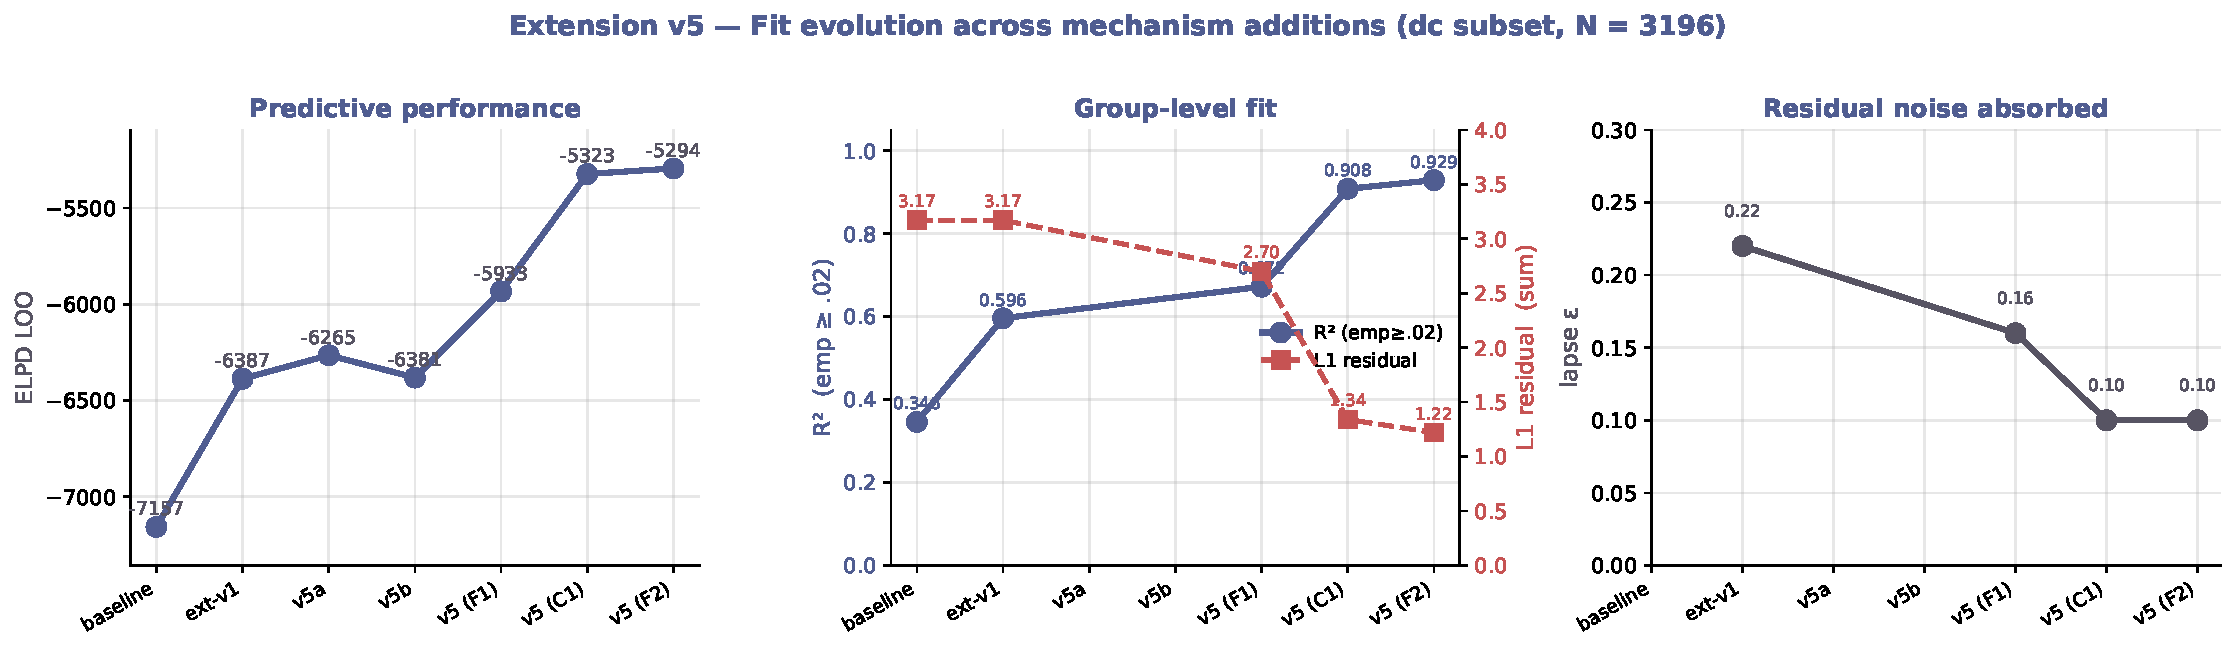
\includegraphics[width=0.97\linewidth]{v5_fit_evolution.pdf}
\end{center}
\vspace{-0.3em}
\footnotesize Each new mechanism shifts LOO and $R^2$ upward and $\varepsilon$ downward. The exception is v5b (saturating $\gamma$ alone), which is flat against ext-v1.
\end{frame}

% ====================================================================
\begin{frame}{Mechanism posteriors across stages}
\vspace{-0.3em}
\begin{center}
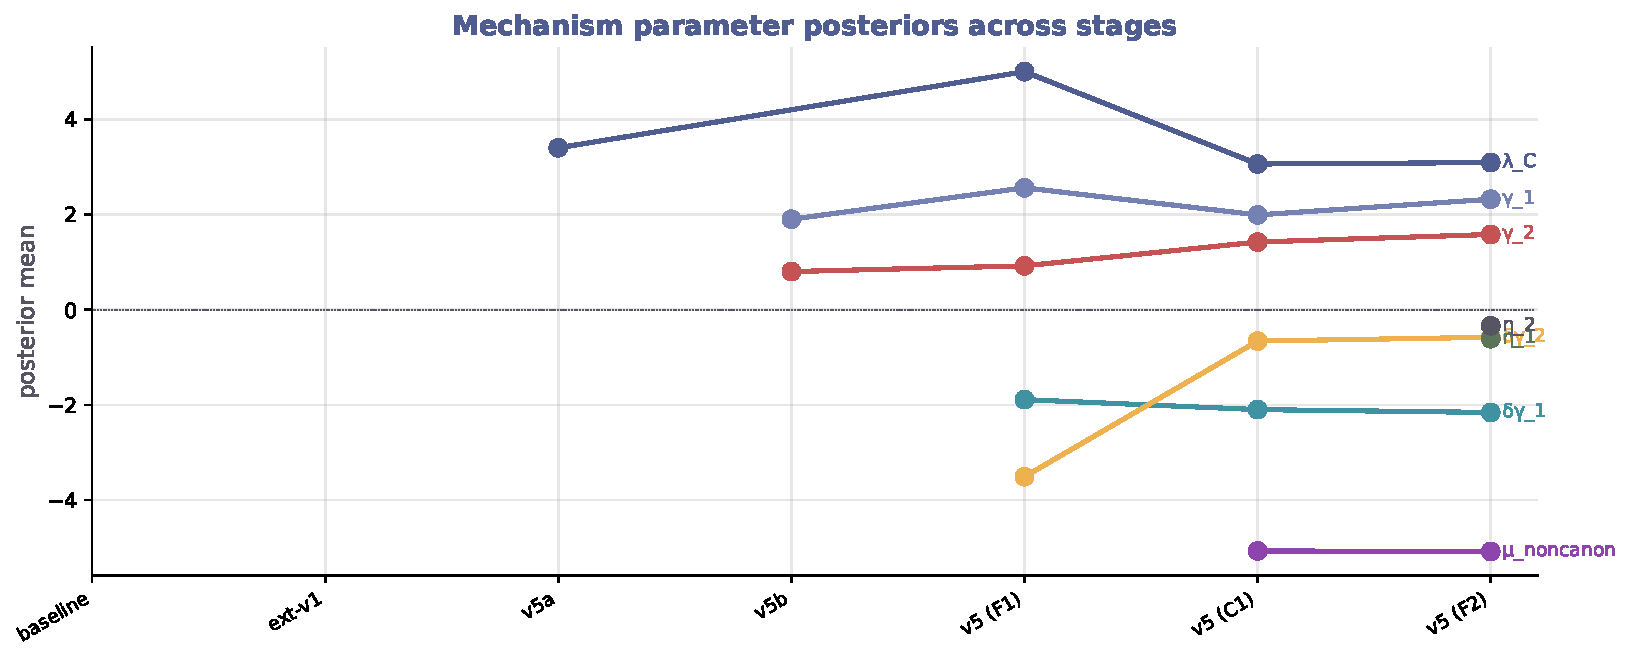
\includegraphics[width=0.97\linewidth]{v5_param_evolution.pdf}
\end{center}
\vspace{-0.3em}
\footnotesize Each mechanism parameter enters with a consistent posterior sign and settles by F2. $\lambda_C$ and $\mu_\mathrm{nc}$ are strong, $\eta$ is modest, $\delta\gamma_1$ is clearly negative on csuff, and $\delta\gamma_2$ shrinks once $\mu_\mathrm{nc}$ absorbs canonical-order variance. $\log\beta$ (dashed) is pre-existing and drops sharply from $\sim 2$ to $-0.18$ once $\mu_\mathrm{nc}$ is added, indicating that canonical ordering absorbs much of what the LM prior was previously encoding.
\end{frame}

% ====================================================================
\begin{frame}{Ablation: is the LM prior still needed under F2?}
\small
Test: fit v5 (F2) with $\beta = 0$, effectively removing the LM prior. Every other mechanism is held fixed.

\vspace{0.6em}
\begin{center}
\begin{tabular}{lrrrr}
\toprule
Model         & ELPD    & $\Delta$ vs F2 & $R^2$ & L1 \\
\midrule
\main{v5 (F2)}   & \main{$-5294$} & $0$     & \main{$.928$} & \main{$1.22$} \\
v5\_no\_lm (F3)  & $-5314$ & $-20.3$ & $.915$ & $1.30$ \\
\bottomrule
\end{tabular}
\end{center}

\vspace{0.6em}
Posterior compensation when the LM prior is removed:
\begin{itemize}\itemsep0.15em
  \item $\lambda_C$: $3.09 \to 3.33$ 
  \item $\gamma_2$: $1.58 \to 1.32$ 
  \item $\delta\gamma_1$: $-2.16 \to -2.39$
  \item $\mu_\mathrm{nc}, \gamma_1, \eta, \varepsilon$: essentially unchanged.
\end{itemize}

\vspace{0.6em}
LM prior contribution goes most likely to frequency structure beyond canonical ordering and length (e.g., relative frequency among same-shape canonical utterances)
\end{frame}

% ====================================================================
\begin{frame}{Final v5 (F2) parameters --- full record}
\small
\begin{center}
\begin{tabular}{lllc}
\toprule
Parameter & Prior & Posterior mean (95\% CI) & $\hat R$\\
\midrule
$\alpha_D$           & HalfN(5)    & (hier.\ w/ $\delta_p$)  & $\leq 1.01$\\
$\alpha_C$           & HalfN(5)    & (hier.)                  & $\leq 1.01$\\
$\alpha_F$           & HalfN(5)    & (hier.)                  & $\leq 1.01$\\
\midrule
$\lambda_C$          & N(0,1)      & \main{$+3.09$} (2.67, 3.55) & 1.00\\
$\gamma_1$           & N(0,1)      & $+2.32$ (2.16, 2.49)     & 1.00\\
$\gamma_2$           & N(0,1)      & $+1.58$ (1.43, 1.74)     & 1.01\\
$\delta\gamma_1$     & N(0,1)      & $-2.16$ (-2.33, -1.97)   & 1.00\\
$\delta\gamma_2$     & N(0,1)      & $-0.58$ (-1.21, +0.04)   & 1.00\\
$\eta_1$             & N(0,1)      & $-0.61$ (-0.77, -0.43)   & 1.00\\
$\eta_2$             & N(0,1)      & $-0.34$ (-0.51, -0.15)   & 1.00\\
$\mu_\mathrm{nc}$    & N(0,1)      & \emp{$-5.08$} (-5.61, -4.56) & 1.01\\
\midrule
$\log\beta$          & N(0,0.5)    & $-0.17$                  & 1.00\\
$\varepsilon$        & Beta(1,50)  & \main{$0.10$} (0.09, 0.12) & 1.00\\
$\tau$               & HalfN(0.2)  & $0.62$ (0.51, 0.73)      & 1.00\\
\bottomrule
\end{tabular}
\end{center}
\end{frame}

% ====================================================================
\begin{frame}{PPC --- v5 (F2) on the dc subset}
\vspace{-0.3em}
\begin{center}
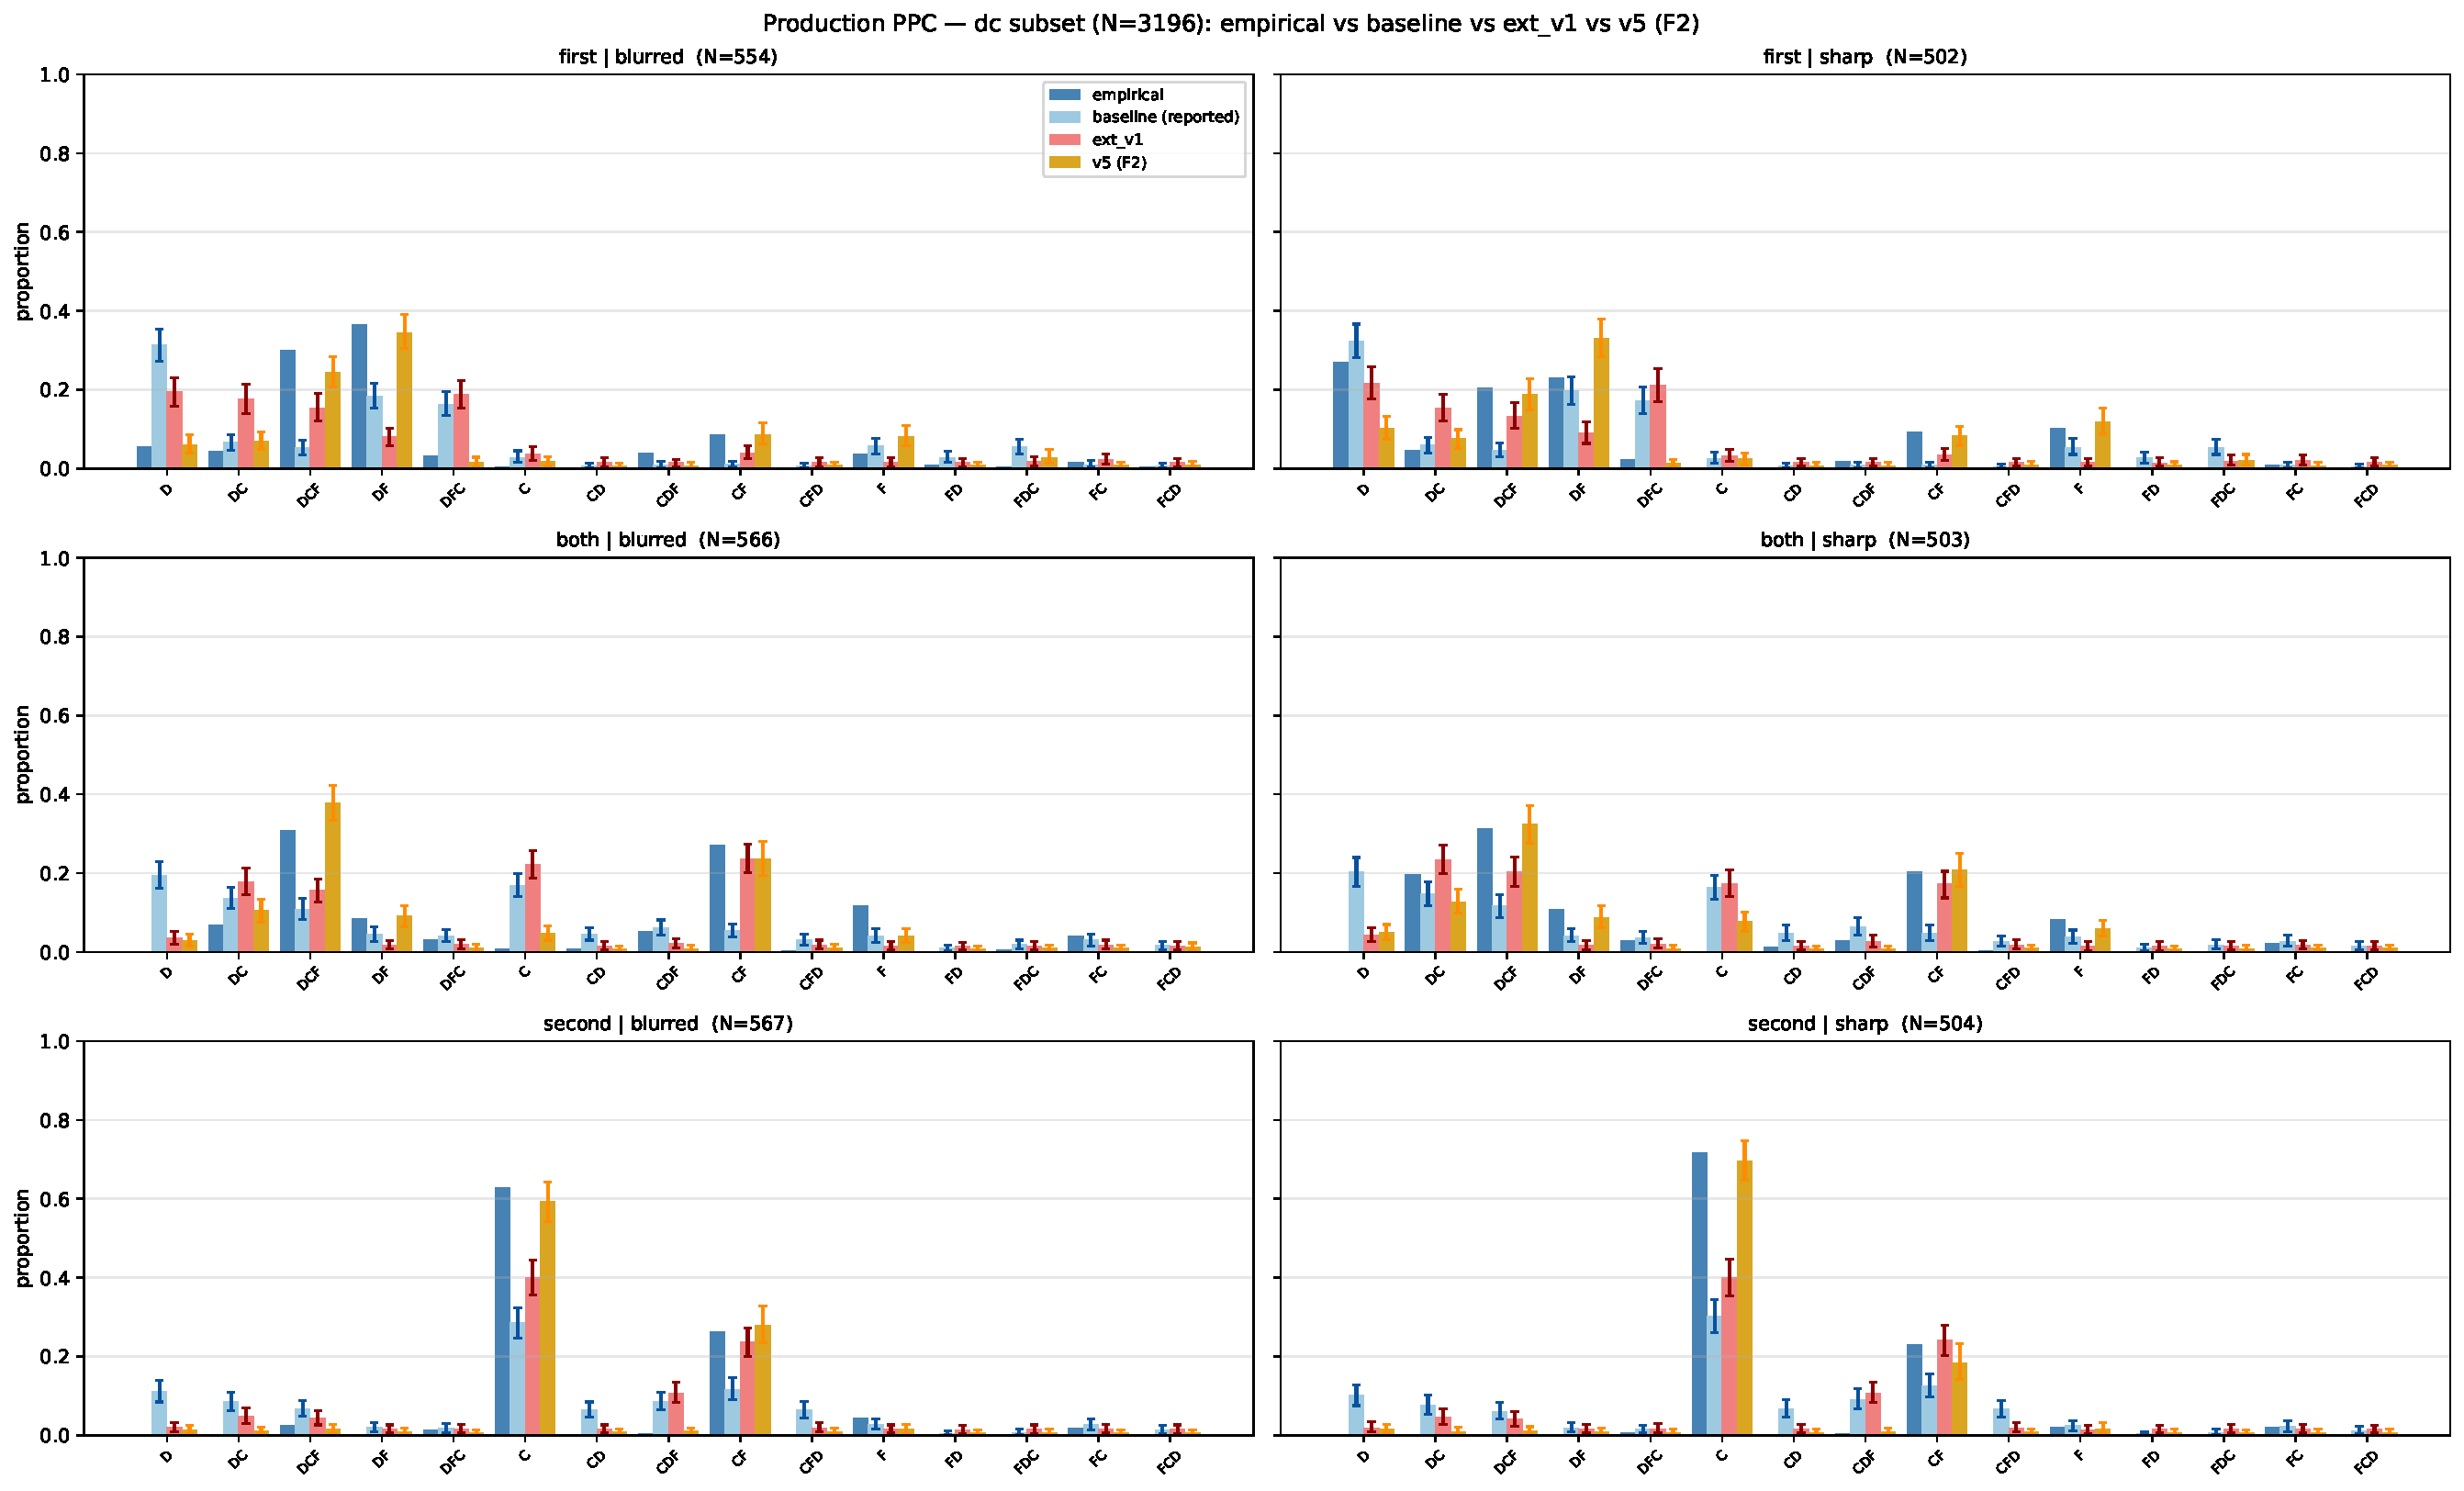
\includegraphics[width=0.96\linewidth]{production_ppc_barplot_v5_dc_F2.pdf}
\end{center}
\vspace{-0.3em}
\footnotesize v5 (F2) posterior predictive on the dc subset ($N = 3196$, $R^2 = .94$). Rows: \texttt{relevant\_property} (\acct{first} / \accg{both} / \accy{second}). Columns: sharpness. v5 F2 (gold) tracks the empirical distribution (blue) across all six cells.
\end{frame}

% ====================================================================
\begin{frame}{Predicted vs observed --- v5 (F2) on the dc subset}
\vspace{-0.3em}
\begin{center}
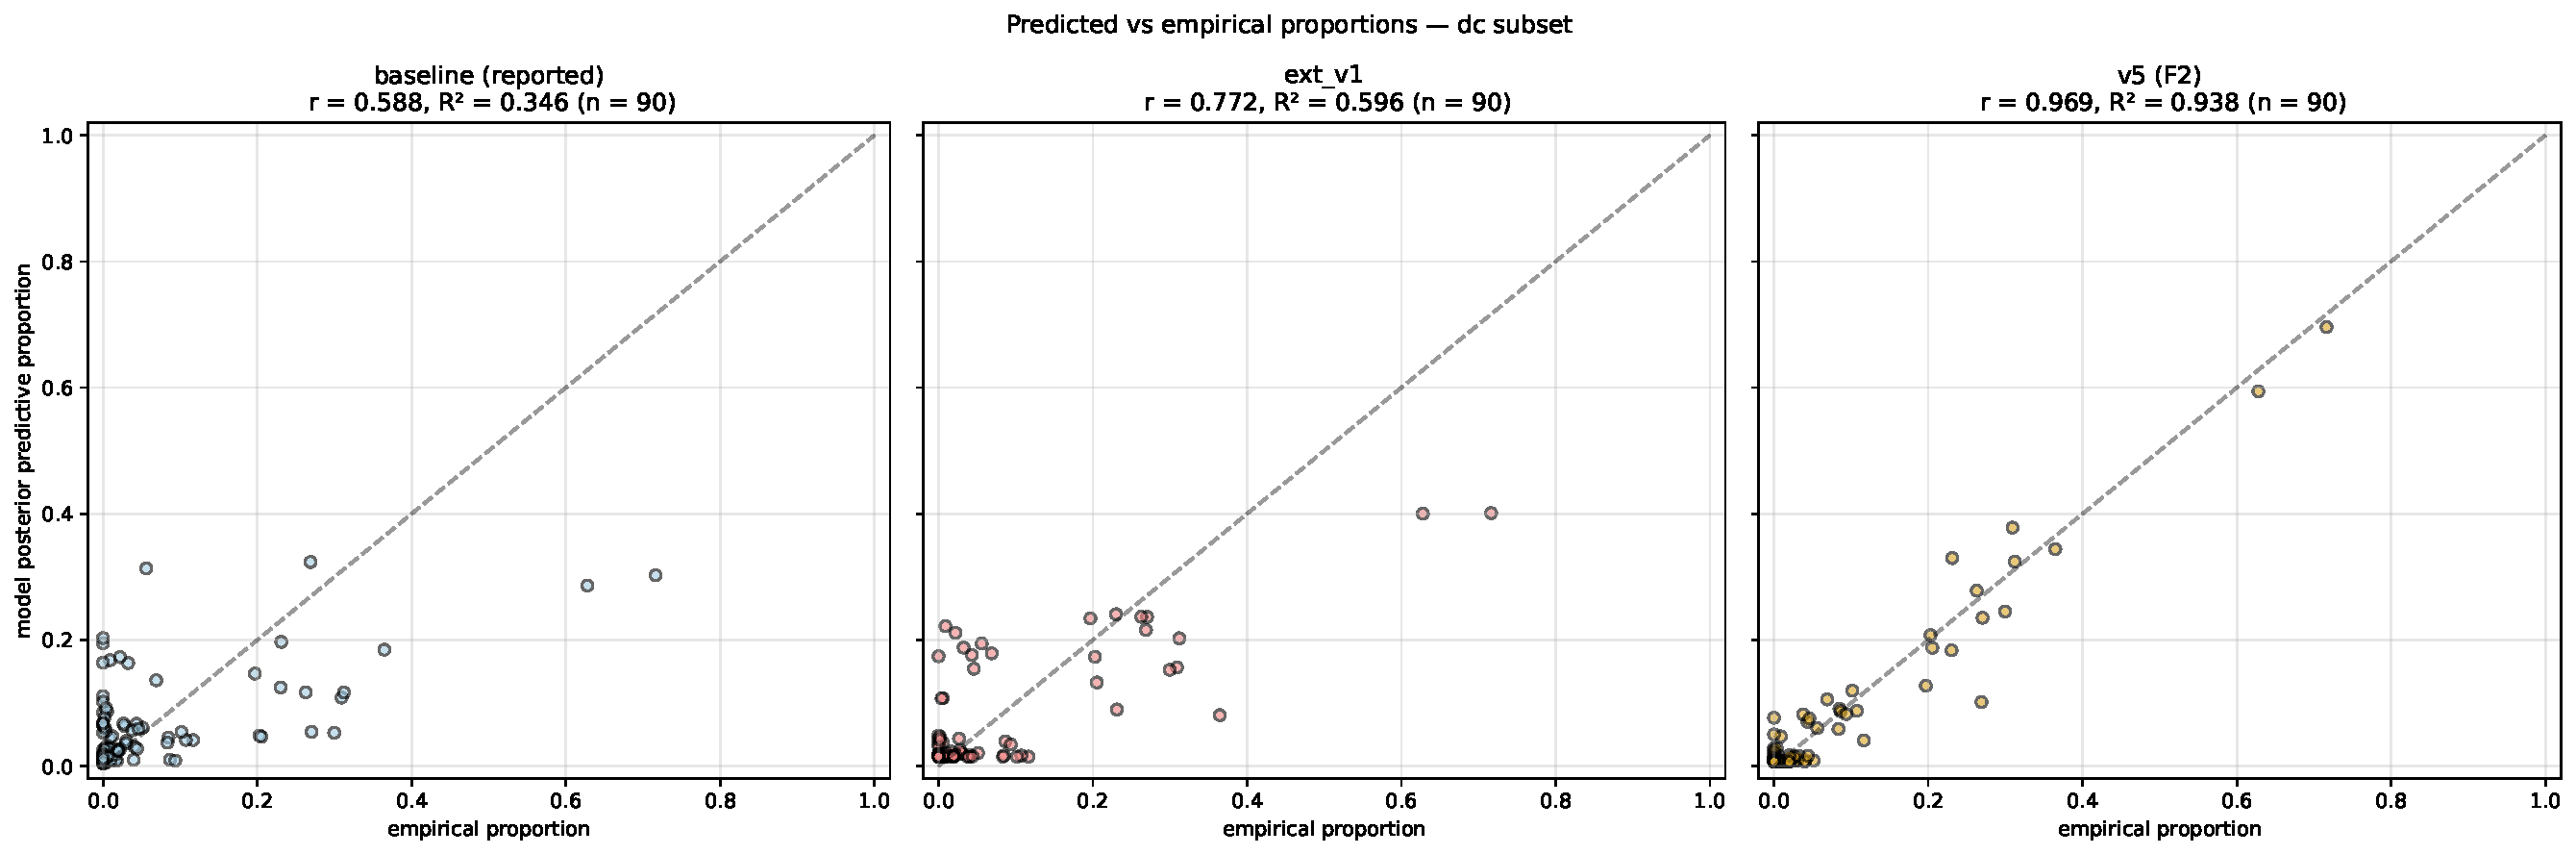
\includegraphics[width=0.98\linewidth]{production_correlation_v5_dc_F2.pdf}
\end{center}
\vspace{-0.3em}
\footnotesize Predicted vs observed proportions across the 30 (condition $\times$ sharpness $\times$ utterance) cells on the dc subset. $R^2$: baseline $.35 \to$ ext-v1 $.60 \to$ \main{v5 (F2) $.94$}.
\end{frame}

% ====================================================================
\begin{frame}{Generalisation to the full data --- proof of concept}
\small
We refit the \emph{same} F2 structure (same mechanisms, same priors, no re-tuning) on the full $N = 9586$ dataset spanning all 9 conditions.

\vspace{0.5em}
\begin{center}\footnotesize
\begin{tabular}{lrrrr}
\toprule
Model          & ELPD LOO & $R^2_{90}$ & $R^2_{270}$ & L1 \\
\midrule
baseline        & $-22703$ & $.10$ & ---   & $6.46$\\
ext-v1          & $-20831$ & $.23$ & ---   & $5.46$\\
\main{v5 (F2)}  & \main{$-15969$} & \main{$.78$} & \main{$.73$} & \main{$2.68$}\\
\bottomrule
\end{tabular}
\end{center}
\footnotesize $R^2_{90}$: 90 (condition-family $\times$ utterance) cells marginalised across sharpness. $R^2_{270}$: full 9 conditions $\times$ 2 sharpness $\times$ 15 utterances.

\vspace{0.5em}
\begin{itemize}\itemsep0.15em
  \item $+4862$ ELPD over ext-v1 on full data (vs.\ $+1093$ on the dc subset) --- the gap widens roughly $4.5\times$.
  \item $\mu_\mathrm{nc}$ posterior: $-5.08$ (dc) $\to$ $-8.30$ (full) --- the canonical-ordering penalty strengthens over the wider condition space.
\end{itemize}

\vspace{0.4em}
\muted{Treat this as a proof of concept rather than a formal out-of-sample test: the mechanisms were designed on the dc subset and refit here, and no posterior checks beyond overall fit metrics have been done yet.}
\end{frame}

% ====================================================================
\begin{frame}{Predicted vs empirical --- full-data fit ($n = 90$ cells marginalised)}
\vspace{-0.3em}
\begin{center}
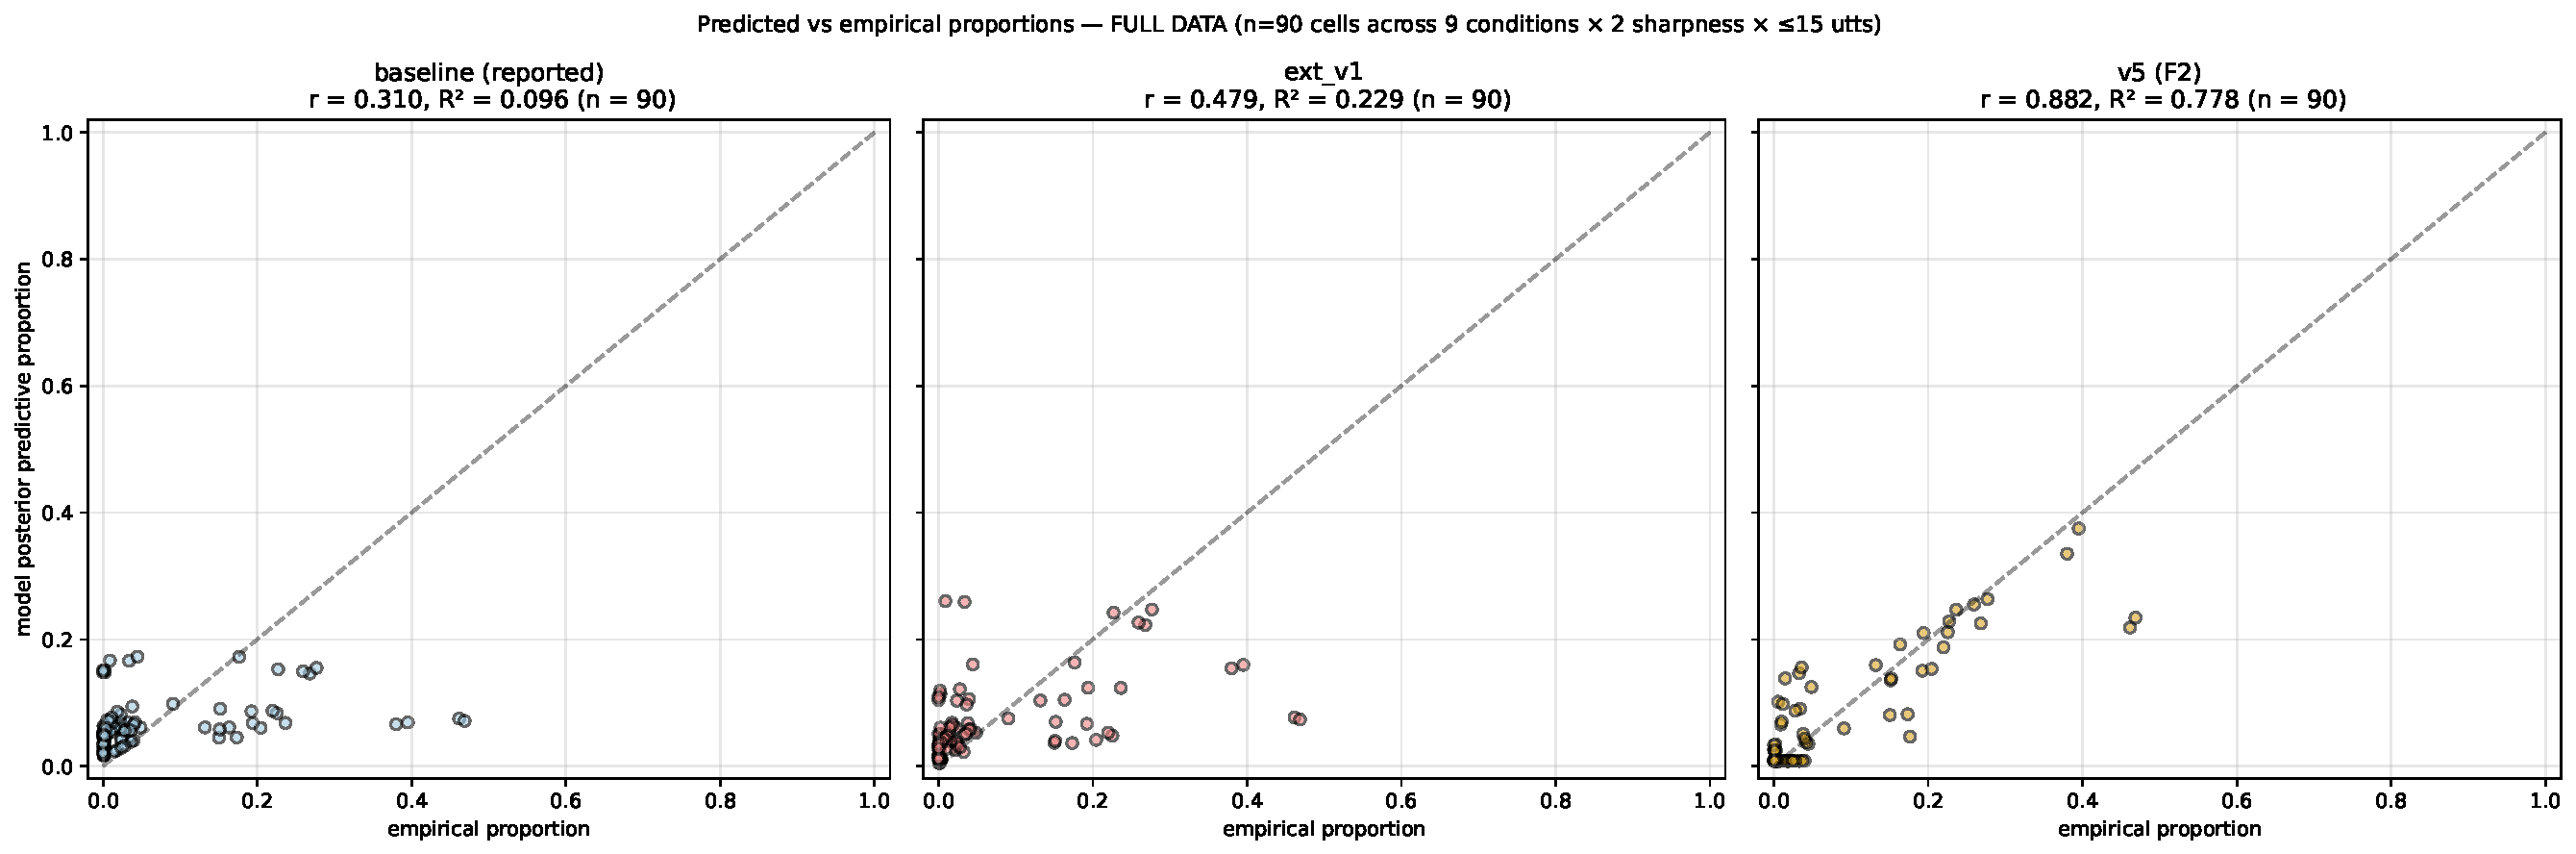
\includegraphics[width=0.98\linewidth]{production_correlation_v5_fulldata_F2.pdf}
\end{center}
\vspace{-0.3em}
\footnotesize All 90 condition-family $\times$ utterance cells. $R^2$: baseline $.10 \to$ ext-v1 $.23 \to$ \main{v5 (F2) $.78$} on full-data fit.
\end{frame}

% ====================================================================
\begin{frame}{Re-running the $2\!\times\!2$ under F2}
With the F2 mechanisms in place, we re-ran the $2\!\times\!2$ (speaker architecture $\times$ semantics regime) on the dc subset.

\vspace{0.8em}
Two parameterisations to compare in the main text:
\begin{enumerate}\itemsep0.3em
  \item Paper-reported: minimal, theory-driven.
  \item F2-full globals: every parameter sampled freely in every cell --- the comparison that holds expressive capacity equal.
\end{enumerate}
\end{frame}
% ====================================================================
\begin{frame}{$2\!\times\!2$ comparison with F2}
\begin{center}
\begin{tabular}{l|rr|r}
\toprule
             & recursive & static & $\Delta$(rec$-$sta) \\
\midrule
incremental  & $-5294$ & $-5297$ & $+2.80$ ($\Delta/$dSE $= 2.22$) \\
global (full)& $-5357$ & $-5365$ & $+8.25$ ($\Delta/$dSE $= 3.82$) \\
\midrule
$\Delta$(inc$-$glb) & $+63$ & $+69$ & \\
$\Delta/$dSE        & \emp{$3.18$} & \emp{$3.48$} & \\
\bottomrule
\end{tabular}
\end{center}

\vspace{0.8em}
Key changes relative to the paper-reported numbers:
\begin{itemize}\itemsep0.2em
  \item Architecture effect $\Delta/$dSE: $11 \to 3.2$ (roughly a third of the paper's).
  \item Regime-within-inc $\Delta/$dSE: $10.28 \to 2.22$ (roughly a fifth of the paper's).
  \item Regime-within-glb: $\approx 0 \to 3.82$ (a modest effect now appears).
  \item Diff-in-diff: $+21 \to -5.45$ --- magnitude shrinks and sign reverses (recursive now helps global slightly more than incremental).
\end{itemize}
\end{frame}

% ====================================================================
\begin{frame}{Full record --- side-by-side}
\small
\begin{center}
\begin{tabular}{lcc}
\toprule
                             & Paper-reported   & \main{F2-full} \\
\midrule
Sampled parameters           & $\alpha, \log\beta, \tau, \delta_p$ & + $\alpha_D\!\mid\!\alpha_C\!\mid\!\alpha_F$ (hier), $\lambda_C$, $\gamma_{1,2}$, $\delta\gamma_{1,2}$, $\eta_{1,2}$, $\mu_\mathrm{nc}$, $\varepsilon$ \\
Fixed                        & $\gamma\!=\!0,\ \varepsilon\!=\!0$   & --- (all of above sampled) \\
\midrule
$R^2$ (all cells)            & $.35$       & \main{$.94$} \\
L1 residual                  & $3.17$      & \main{$1.22$} \\
Lapse $\varepsilon$          & $0$ (fixed) & $0.10$ (sampled) \\
\midrule
Arch effect $\Delta/$dSE     & $\pm 11$    & $\pm 3.2$ \\
Regime $|$inc $\Delta/$dSE   & $10.28$     & $2.22$ \\
Regime $|$glb $\Delta/$dSE   & $\approx 0$ & $3.82$ \\
Interaction (diff-in-diff)   & $+21$       & $-5.45$ \\
\midrule
Rec helps\ldots              & incremental & slightly global \\
\bottomrule
\end{tabular}
\end{center}

\vspace{0.6em}
\footnotesize \muted{F2-full adds 9 sampled mechanism parameters on top of the paper-reported set, plus per-dim hierarchical $\alpha$ and a sampled lapse. The F2-fixed parameterisation (globals frozen at inc-recursive posterior means) is moved to the appendix.}
\end{frame}

% ====================================================================
\begin{frame}{The tradeoff between the two tracks}
\begin{columns}[t]
\begin{column}{0.48\textwidth}
Theory track (paper):
\begin{itemize}\itemsep0.2em
  \item Minimal, motivated mechanisms.
  \item Clear $2\!\times\!2$ interaction.
  \item Group-level fit is poor ($R^2 = .35$).
  \item Seven large misfits in \S5.3.
  \item Lapse absorbs unexplained structure.
\end{itemize}
\end{column}

\begin{column}{0.48\textwidth}
Mechanism track (F2):
\begin{itemize}\itemsep0.2em
  \item Richer; each term is literature-motivated.
  \item Much better fit ($R^2 = .94$).
  \item All seven misfits resolved.
  \item Lapse halved ($0.22 \to 0.10$).
  \item Architecture signal shrinks to $\Delta/$dSE $= 3$.
  \item Regime-within-inc weakens to marginal.
\end{itemize}
\end{column}
\end{columns}

\vspace{1em}
The mechanisms we added to reduce residuals also absorb variance that the paper's minimal parameterisation had attributed to architecture $\times$ regime. The interaction survives, but in reduced form.
\end{frame}

% ====================================================================
\begin{frame}{Two readings of the tradeoff}
\small
Reading I --- the mechanisms are rivals to the architectural account.

The paper's interaction was partly architectural sparsity fitting error structure. Once the error is absorbed by explicit mechanisms (colour salience, canonical ordering, context-dependent length), the residual architectural signal is modest, and the main claim has to be weakened accordingly.

\vspace{1em}
Reading II --- the mechanisms are what the architecture was \emph{supposed} to capture but fails to.

$\lambda_C$, $\mu_\mathrm{nc}$, $\delta\gamma$, and $\eta$ are all condition-dependent context effects --- exactly the kind of structure that a context-updating incremental speaker was introduced to model. On this reading the architecture fails in practice for one of two reasons: (i) the context signal is too subtle for threshold updates to pick up (the architecture exists but is not sensitive enough), or (ii) human behaviour is qualitatively different from what threshold updates predict (e.g., a first-step colour boost or a canonical-order preference that no threshold update can reproduce). Either way, making these mechanisms explicit is how the model starts tracking the context the architecture was meant to track.

\vspace{1em}
Both readings are compatible with the numbers; the choice is mainly a question of how we want to frame the paper.
\end{frame}
% ====================================================================
\begin{frame}{Summary}
\small
\begin{itemize}\itemsep0.3em
  \item The paper-reported model is theory-driven and yields an interpretable $2\!\times\!2$, but the fit is poor ($R^2 = .35$).
  \item The residuals trace to three largely independent phenomena: colour salience, canonical ordering, and condition-dependent length bias.
  \item Adding all three (v5 F2) lifts the fit to $R^2 = .94$ and brings the lapse down to $.10$, with every new parameter credibly non-zero and 0 divergences.
  \item Re-running the $2\!\times\!2$ under F2: the architecture effect shrinks by roughly a factor of three, and the regime effect shrinks and partially flips direction.
\end{itemize}

\vspace{1em}
\end{frame}

% ====================================================================
\begin{frame}{Thanks}
\centering
\vspace{2em}
\Large Questions and discussion.

\vspace{2em}
\normalsize
\end{frame}

% ====================================================================
\begin{frame}{Appendix: paper-reported model parametrization}
\small
\main{Sampled parameters.}
\begin{center}\footnotesize
\begin{tabular}{lll}
\toprule
Parameter & Role & Prior \\
\midrule
$\alpha$      & rationality (shared across D, C, F)           & $\mathrm{HalfNormal}(5.0)$ \\
$\log\beta$   & LM prior weight, $\beta = \exp(\log\beta)$    & $\mathrm{Normal}(0,\, 0.5)$ \\
$\tau$        & participant random-effect scale on $\alpha$   & $\mathrm{HalfNormal}(0.2)$ \\
$\delta_p$    & per-participant offset on $\alpha$            & $\mathrm{Normal}(0,\, \tau)$ \\
\bottomrule
\end{tabular}
\end{center}

\vspace{0.5em}
\main{Fixed (not sampled) parameters.}
\begin{center}\footnotesize
\begin{tabular}{lll}
\toprule
Parameter & Role & Value \\
\midrule
$\gamma$            & length bias                              & $0$ \\
$\varepsilon$       & lapse                                    & $0$ \\
$k$                 & size threshold                           & $0.5$ \\
$w_f$               & form weight                              & $1.0$ \\
$\nu_\text{colour}$ & colour semantic value                    & $0.85$ \\
$\nu_\text{form}$   & form semantic value (production only)    & $0.70$ \\
\bottomrule
\end{tabular}
\end{center}

\vspace{0.5em}
\main{MCMC settings (NumPyro NUTS).}
\begin{itemize}\itemsep0.1em
  \item 4 chains, $5{,}000$ warmup and $2{,}000$ post-warmup samples per chain.
  \item Target acceptance probability $= 0.85$, maximum tree depth $= 7$.
  \item Convergence confirmed via split-$\hat R < 1.01$ and $n_\text{eff} > 400$ across all parameters.
\end{itemize}

\vspace{0.4em}
\muted{Note: the extension track (ext-v1 $\to$ v5 F2) uses the code defaults $\nu_\text{colour} = 0.971$, $\nu_\text{form} = 0.50$; the paper-reported Set B values shown here are $0.85$ and $0.70$.}
\end{frame}

% ====================================================================
\begin{frame}{Appendix: why not free the semantic parameters?}
\small
An alternative to the mechanism track is to sample $k$, $\nu_\text{colour}$, $\nu_\text{form}$, and $w_f$ instead of fixing them. These parameters directly control the utility imbalance behind the residuals (currently colour $\approx 1.65$ nats, size $\approx 0.06$ nats, form $\approx 0$ nats).

\vspace{0.4em}
\main{Identifiability --- profile-posterior analysis (Feb 2026).}
\begin{itemize}\itemsep0.1em
  \item $k$ is not identifiable: the profile posterior is flat, because the size manipulation is not contrastive enough to pin $k$ down.
  \item $\nu_\text{colour}$ and $\nu_\text{form}$ are each unimodal individually, but the joint posterior is bimodal and NUTS chains do not mix.
  \item $w_f$: sharpening (lower $w_f$) consistently hurts in grid search.
\end{itemize}

\vspace{0.4em}
\main{Grid search over fixed values (March 2026).}
\begin{itemize}\itemsep0.1em
  \item Lowering $\nu_\text{colour}$ from $0.971$ to $0.85$ is the only change that helps: $+137$ ELPD on the reported model (3-cond subset), $+245$ on full data, with $p_\text{loo}$ dropping from $93$ to $67$.
  \item Form and size-sharpness variations are negligible or harmful.
\end{itemize}

\vspace{0.4em}
The semantic parameters are therefore not jointly identifiable, so freeing them is not a viable substitute for the mechanism track. Fixed-value search points in the same qualitative direction --- colour's effective discriminability should be lower than its literal reading --- and v5 adds identifiable handles on top of this fixed-representation baseline.
\end{frame}

% ====================================================================
\begin{frame}{Appendix: $2\!\times\!2$ with F2 globals fixed at inc-recursive means}
\small
Sanity-check parameterisation: the global cells use $\gamma, \delta\gamma, \eta, \mu_\mathrm{nc}$ fixed at the incremental-recursive posterior means, rather than sampled freely.

\vspace{0.6em}
\begin{center}
\begin{tabular}{l|rr|r}
\toprule
              & recursive & static & $\Delta$(rec$-$sta) \\
\midrule
incremental   & $-5294$ & $-5297$ & $+2.80$ ($\Delta/$dSE $= 2.22$, marginal) \\
global (fixed)& $-5600$ & $-5619$ & \emp{$+19.15$} ($\Delta/$dSE $= 6.99$) \\
\midrule
$\Delta$(inc$-$glb) & $+306$ & $+323$ & \\
$\Delta/$dSE        & $10.51$ & $11.03$ & \\
\bottomrule
\end{tabular}
\end{center}

\vspace{0.6em}
\begin{itemize}\itemsep0.15em
  \item The architecture effect is still large ($\Delta/$dSE $\approx 10.5$).
  \item The interaction has flipped: recursive now helps global, not incremental.
  \item This is not a like-for-like test --- the global models are constrained to inc-recursive parameter values. F2-full globals is the fair comparison.
\end{itemize}
\end{frame}

% ====================================================================
\begin{frame}{Appendix: full LOO \& fit record --- all stages}
\footnotesize
\begin{center}
\begin{tabular}{l rrrr rr}
\toprule
Stage & ELPD LOO & $\Delta$ vs baseline & $\Delta$ vs ext-v1 & $R^2$ & L1 & $\varepsilon$ \\
\midrule
baseline        & $-7157$ & $0$       & ---       & $.35$ & $3.17$ & ---   \\
ext-v1          & $-6387$ & $+770$    & $0$       & $.60$ & $3.17$ & $.23$  \\
\muted{v2 (first-word intercepts) --- rejected}  & $-6337$ & $+820$  & $+50$   & $.62$ & ---     & ---   \\
\muted{v3 (step-level $\mu$, per-dim $\alpha$) --- rejected} & \multicolumn{6}{l}{non-identifiable ($\hat R \leq 14.7$)} \\
\muted{v4 (step-level $\mu$, single $\alpha$) --- rejected} & $-6449$ & $+708$  & $-62$   & $.54$ & ---     & ---   \\
\acct{v5a ($\lambda_C$ only)}         & $-6265$ & $+892$  & $+122$   & ---   & ---     & ---   \\
\acct{v5b (sat.\ $\gamma$ only)}      & $-6381$ & $+776$  & $+6$     & ---   & ---     & ---   \\
\main{v5 (F1: $\lambda_C + \delta\gamma$)}   & $-5933$ & $+1224$ & $+454$   & $.67$ & $2.70$  & $.16$ \\
\main{v5 (C1: + $\mu_\mathrm{nc}$)}          & $-5323$ & $+1834$ & $+1063$  & $.91$ & $1.34$  & $.10$ \\
\emp{v5 (F2: + $\eta$)}                      & $-5294$ & $+1863$ & $+1093$  & $.94$ & $1.22$  & $.10$ \\
\muted{v5\_no\_lm (F3: F2 with $\beta=0$)}     & $-5314$ & $+1843$ & $+1073$  & $.92$ & $1.30$  & $.10$ \\
\midrule
\multicolumn{7}{l}{\textit{Full data generalization check (N = 9586, all 9 conditions):}} \\
\muted{baseline \ (full data)}              & $-22703$ & $0$      & ---      & $.10$ & $6.46$  & ---   \\
\muted{ext-v1 \ \ \ (full data)}            & $-20831$ & $+1872$  & $0$      & $.23$ & $5.46$  & $.05$ \\
\main{v5 (F2, full data)}                   & $-15969$ & $+6734$  & $+4862$  & $.78$ & $2.68$  & $.12$ \\
\bottomrule
\end{tabular}
\end{center}

\vspace{0.6em}
\begin{itemize}\itemsep0.15em
  \item Columns: LOO, $R^2$ over cells with empirical $\geq .02$, L1 (sum of $|\Delta|$ over 37 cells), and posterior mean of $\varepsilon$.
  \item Baseline has no lapse and no length bias: $\gamma$ and $\varepsilon$ are hardcoded to $0$ in \texttt{likelihood\_function\_reported\_hier}, not sampled. Entries marked ``---'' are structurally absent, not unreported.
  \item v2--v4: rejected exploratory variants.
  \item v5a and v5b: isolated mechanism probes (no full $R^2$/L1 computed).
  \item Each add-on moves the metrics in the expected direction, with two exceptions: v5b (saturating $\gamma$ alone, null) and v4 (worse than ext-v1).
  \item F3 (LM prior removed): $-20$ ELPD vs.\ F2. The LM prior still contributes beyond $\mu_\mathrm{nc} + \gamma$, so we keep it.
  \item Full-data generalisation: v5 F2 fit on all $N=9586$ gives $+4862$ ELPD over ext-v1 (vs.\ $+1093$ on the dc subset) --- a roughly $4.5\times$ larger gap. $R^2 = .78$ on 90 marginalised cells.
  \item $\mu_\mathrm{noncanon}$ posterior: $-5.08$ (dc) $\to$ $-8.30$ (full data), indicating a stronger canonical-ordering penalty on the full 9-condition data.
\end{itemize}
\end{frame}

% ====================================================================
\begin{frame}{Appendix: full parameter record --- posterior means across stages}
\scriptsize
\begin{center}
\renewcommand{\arraystretch}{1.10}
\begin{tabular}{l cc cc ccccc}
\toprule
Parameter & baseline & ext-v1 & \muted{v2} & \muted{v4} & v5a & v5b & v5 (F1) & v5 (C1) & v5 (F2) \\
\midrule
$\alpha_D$           & single $\alpha$ & $6.92$ & $\sim 6.9$ & single $\alpha$ & $\sim 6.9$ & $\sim 6.9$ & hier. & hier. & hier. \\
$\alpha_C$           &                 & $1.85$ & $\sim 1.8$ &                 & $\sim 1.8$ & $\sim 1.9$ & hier. & hier. & hier. \\
$\alpha_F$           &                 & $1.89$ & $\sim 1.9$ &                 & $\sim 1.9$ & $\sim 1.9$ & hier. & hier. & hier. \\
\midrule
$\phi_C$ (first-word) & ---   & ---    & \emp{$-6.89$} & ---    & ---   & ---    & ---    & ---    & ---     \\
$\phi_F$ (first-word) & ---   & ---    & \emp{$-5.90$} & ---    & ---   & ---    & ---    & ---    & ---     \\
$\mu_C$ (step-level)  & ---   & ---    & ---    & fitted & ---   & ---    & ---    & ---    & ---     \\
$\mu_F$ (step-level)  & ---   & ---    & ---    & fitted & ---   & ---    & ---    & ---    & ---     \\
\midrule
$\lambda_C$           & ---   & ---    & ---    & ---    & \main{$+3.4$} & ---    & \main{$+5.0$} & \main{$+3.06$} & \main{$+3.09$} \\
$\gamma$ (linear)     & ---   & $2.31$ & $\sim 2$ & $\sim 2$ & ---   & ---    & ---    & ---    & ---    \\
$\gamma_1$            & ---   & ---    & ---    & ---    & ---   & $+1.9$ & $+2.56$ & $+1.99$ & $+2.32$ \\
$\gamma_2$            & ---   & ---    & ---    & ---    & ---   & $+0.8$ & $+0.92$ & $+1.42$ & $+1.58$ \\
$\delta\gamma_1$      & ---   & ---    & ---    & ---    & ---   & ---    & $-1.89$ & $-2.10$ & $-2.16$ \\
$\delta\gamma_2$      & ---   & ---    & ---    & ---    & ---   & ---    & $-3.51$ & $-0.66$ & $-0.58$ \\
$\eta_1$              & ---   & ---    & ---    & ---    & ---   & ---    & ---    & ---    & $-0.61$ \\
$\eta_2$              & ---   & ---    & ---    & ---    & ---   & ---    & ---    & ---    & $-0.34$ \\
$\mu_\mathrm{nc}$     & ---   & ---    & ---    & ---    & ---   & ---    & ---    & \emp{$-5.07$} & \emp{$-5.08$} \\
\midrule
$\log\beta$           & $\sim 2$ & $2.05$ & $\sim 2$ & $\sim 2$ & $\sim 2$ & $\sim 2$ & $2.05$ & $-0.18$ & $-0.17$ \\
$\varepsilon$         & ---   & $0.23$ & $\sim .2$ & $\sim .2$ & ---      & ---      & $0.16$ & $0.10$ & $0.10$ \\
$\tau$                & ---   & $0.92$ & ---    & ---    & ---   & ---    & $0.94$ & $0.60$ & $0.62$ \\
\bottomrule
\end{tabular}
\end{center}

{\scriptsize \muted{v3 omitted (non-identifiable).}}

\vspace{0.5em}
\scriptsize
\begin{itemize}\itemsep0.1em
  \item \muted{``hier.''} = $\alpha$ sampled hierarchically with per-participant $\delta_p$; population means close to ext-v1's values.
  \item Each new parameter enters with a consistent sign and keeps it across subsequent stages.
  \item $\log\beta$ drops sharply once $\mu_\mathrm{nc}$ is added --- canonical ordering absorbs what the LM prior was partially encoding.
  \item $\delta\gamma_2$ shrinks from $-3.51$ (F1) to $\sim\!-0.6$ (C1/F2) --- $\mu_\mathrm{nc}$ and $\eta$ absorb part of the 3-word penalty.
\end{itemize}
\end{frame}

% ====================================================================
\begin{frame}{Appendix: ext-v1 posterior predictive check}
\vspace{-0.3em}
\begin{center}
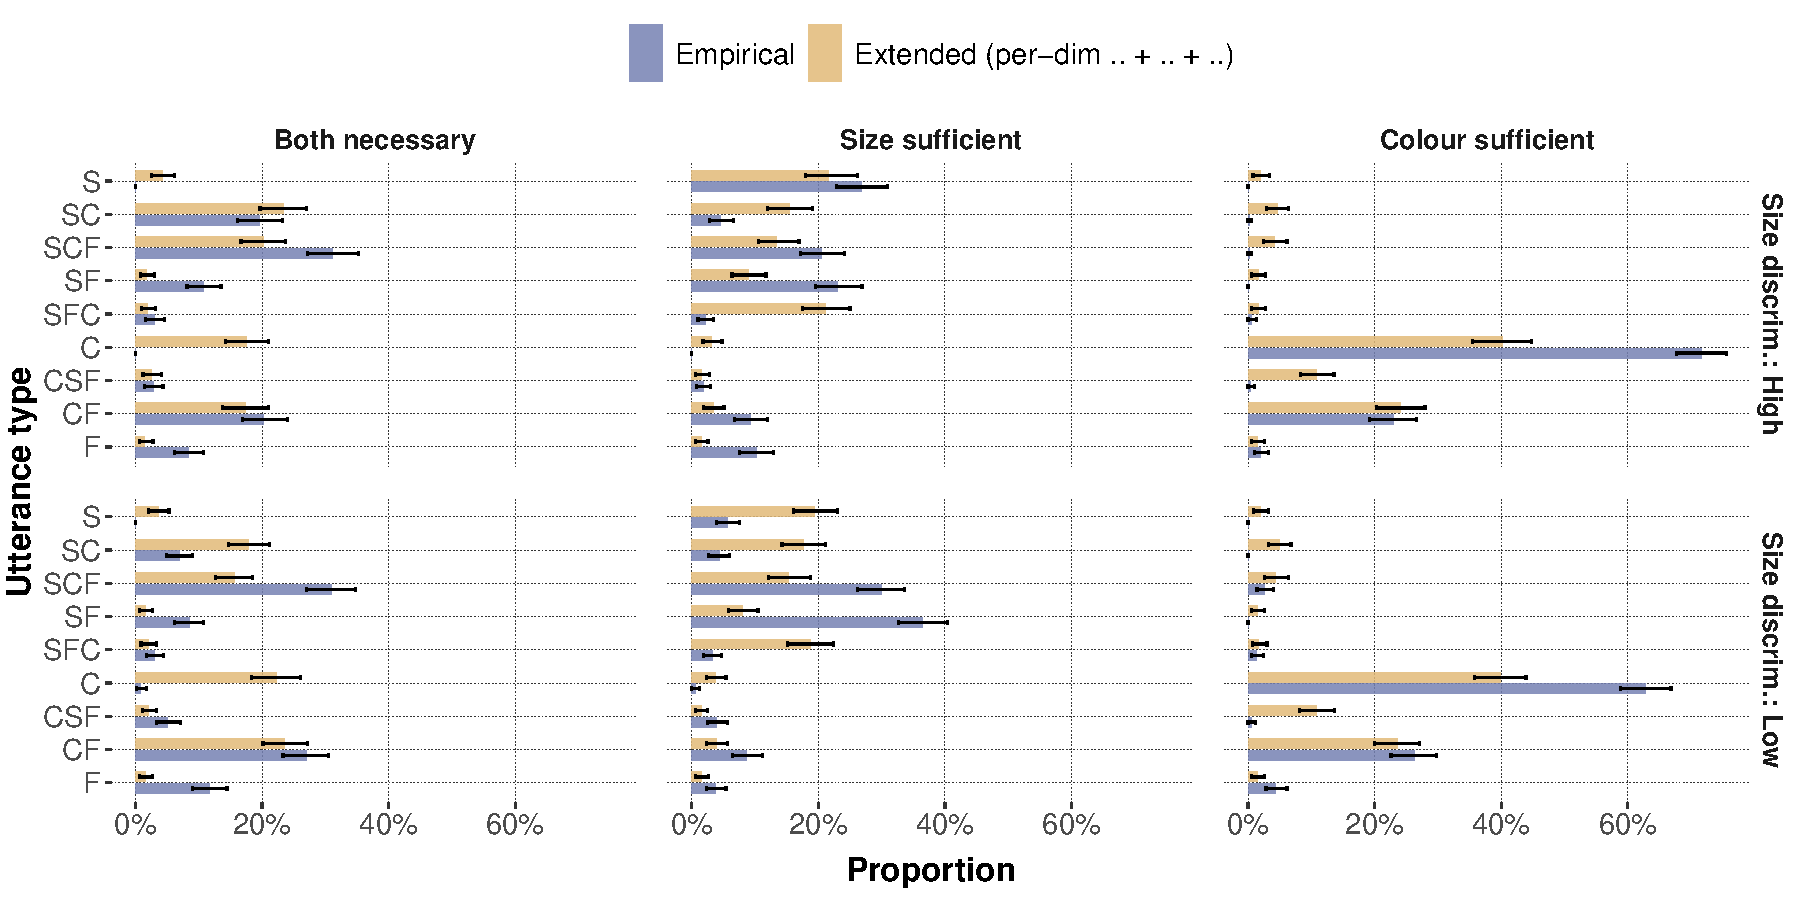
\includegraphics[width=0.82\linewidth]{production_ppc_barplot_extended_v1.pdf}
\end{center}
\vspace{0.2em}
\footnotesize
Empirical (blue) vs ext-v1 predicted (gold) utterance proportions by condition $\times$ sharpness. Per-dim $\alpha$ and explicit $\gamma$ lift bare C in colour-sufficient and recover some mass on CF and DCF; residual misfits remain.
\end{frame}

% ====================================================================
\begin{frame}{Appendix: ext-v1 predicted vs observed}
\vspace{-0.3em}
\begin{center}
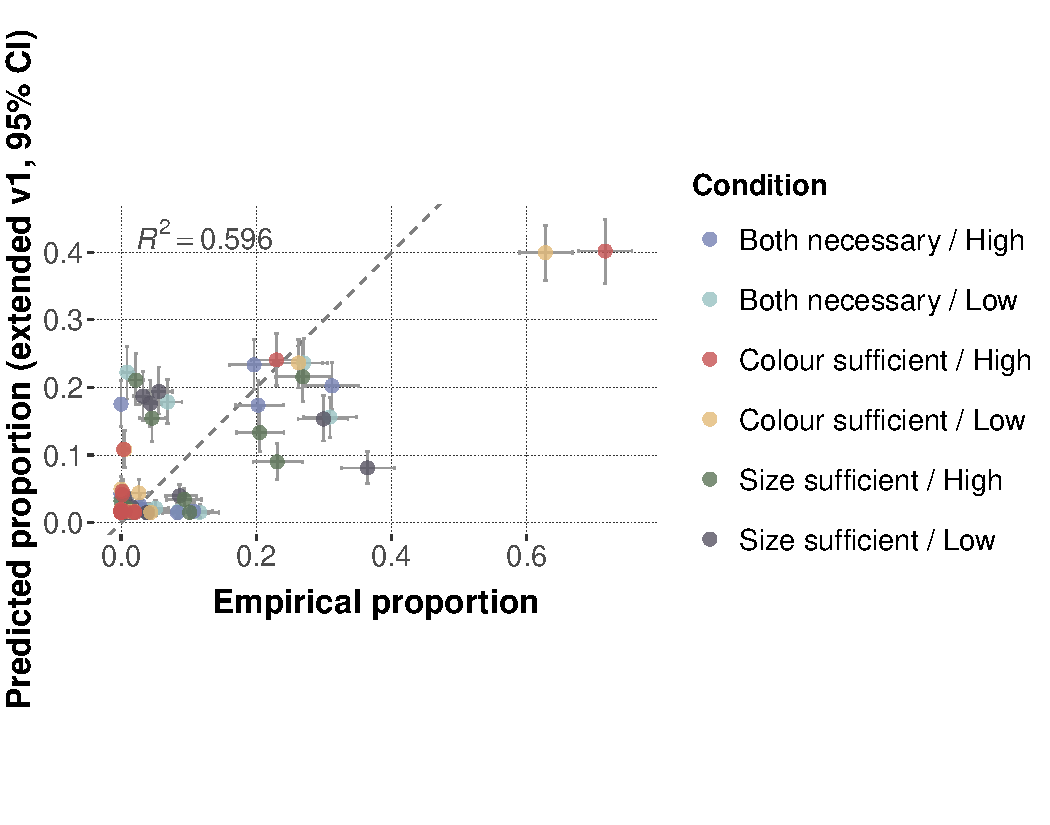
\includegraphics[width=0.58\linewidth]{production_correlation_extended_v1.pdf}
\end{center}
\vspace{0.2em}
\footnotesize
Predicted vs observed across all 90 condition $\times$ utterance cells. $R^2$ improves from $.41$ (paper-reported) to $.60$.
\end{frame}

% ====================================================================
\begin{frame}{Appendix: ext-v1 --- what improved and what persists}
\small
\main{What the extension closes.}
\begin{itemize}\itemsep0.1em
  \item Per-dim $\alpha$ ($\alpha_C = 1.85$ vs.\ the reported single $\alpha \approx 1.0$) partially lifts bare C in colour-sufficient.
  \item Explicit $\gamma = 2.31$ gives multi-adjective utterances (CF, DCF) a utility boost, closing most of the bare-D over-prediction seen in the paper-reported model.
  \item Lapse $\varepsilon = 0.23$ absorbs the remainder.
\end{itemize}

\vspace{0.4em}
\main{Residuals that persist (seven largest).}
\begin{center}\footnotesize
\begin{tabular}{lll rrr}
\toprule
Condition & Sharpness & Utterance & Emp & ext-v1 & $\Delta$\\
\midrule
colour-sufficient & high & C   & .716 & .402 & $\emp{-.314}$\\
colour-sufficient & low  & C   & .628 & .399 & $\emp{-.229}$\\
both-necessary    & low  & C   & .009 & .222 & $\emp{+.213}$\\
both-necessary    & high & C   & .000 & .175 & $\emp{+.175}$\\
size-sufficient   & low  & DF  & .365 & .081 & $\emp{-.284}$\\
size-sufficient   & high & DFC & .022 & .208 & $\emp{+.186}$\\
size-sufficient   & low  & DFC & .032 & .187 & $\emp{+.155}$\\
\bottomrule
\end{tabular}
\end{center}

\vspace{0.4em}
Two diagnostic axes remain:
\begin{itemize}\itemsep0.1em
  \item Bare C is still context-dependent: under-predicted in colour-sufficient and over-predicted in both-necessary. A condition-independent $\alpha_C$ cannot flip sign across contexts.
  \item Length residuals saturate: DF under-predicted in blurred size-sufficient, DFC over-predicted in size-sufficient --- no monotone scalar $\gamma$ fits both.
\end{itemize}

\vspace{0.3em}
These motivate the v5 track: condition-gated $\lambda_C$, saturating $\gamma_1/\gamma_2$, and condition-dependent $\delta\gamma$.
\end{frame}

% ====================================================================
\begin{frame}{Appendix: full-data F2 fit displayed on dc cells}
\vspace{-0.3em}
\begin{center}
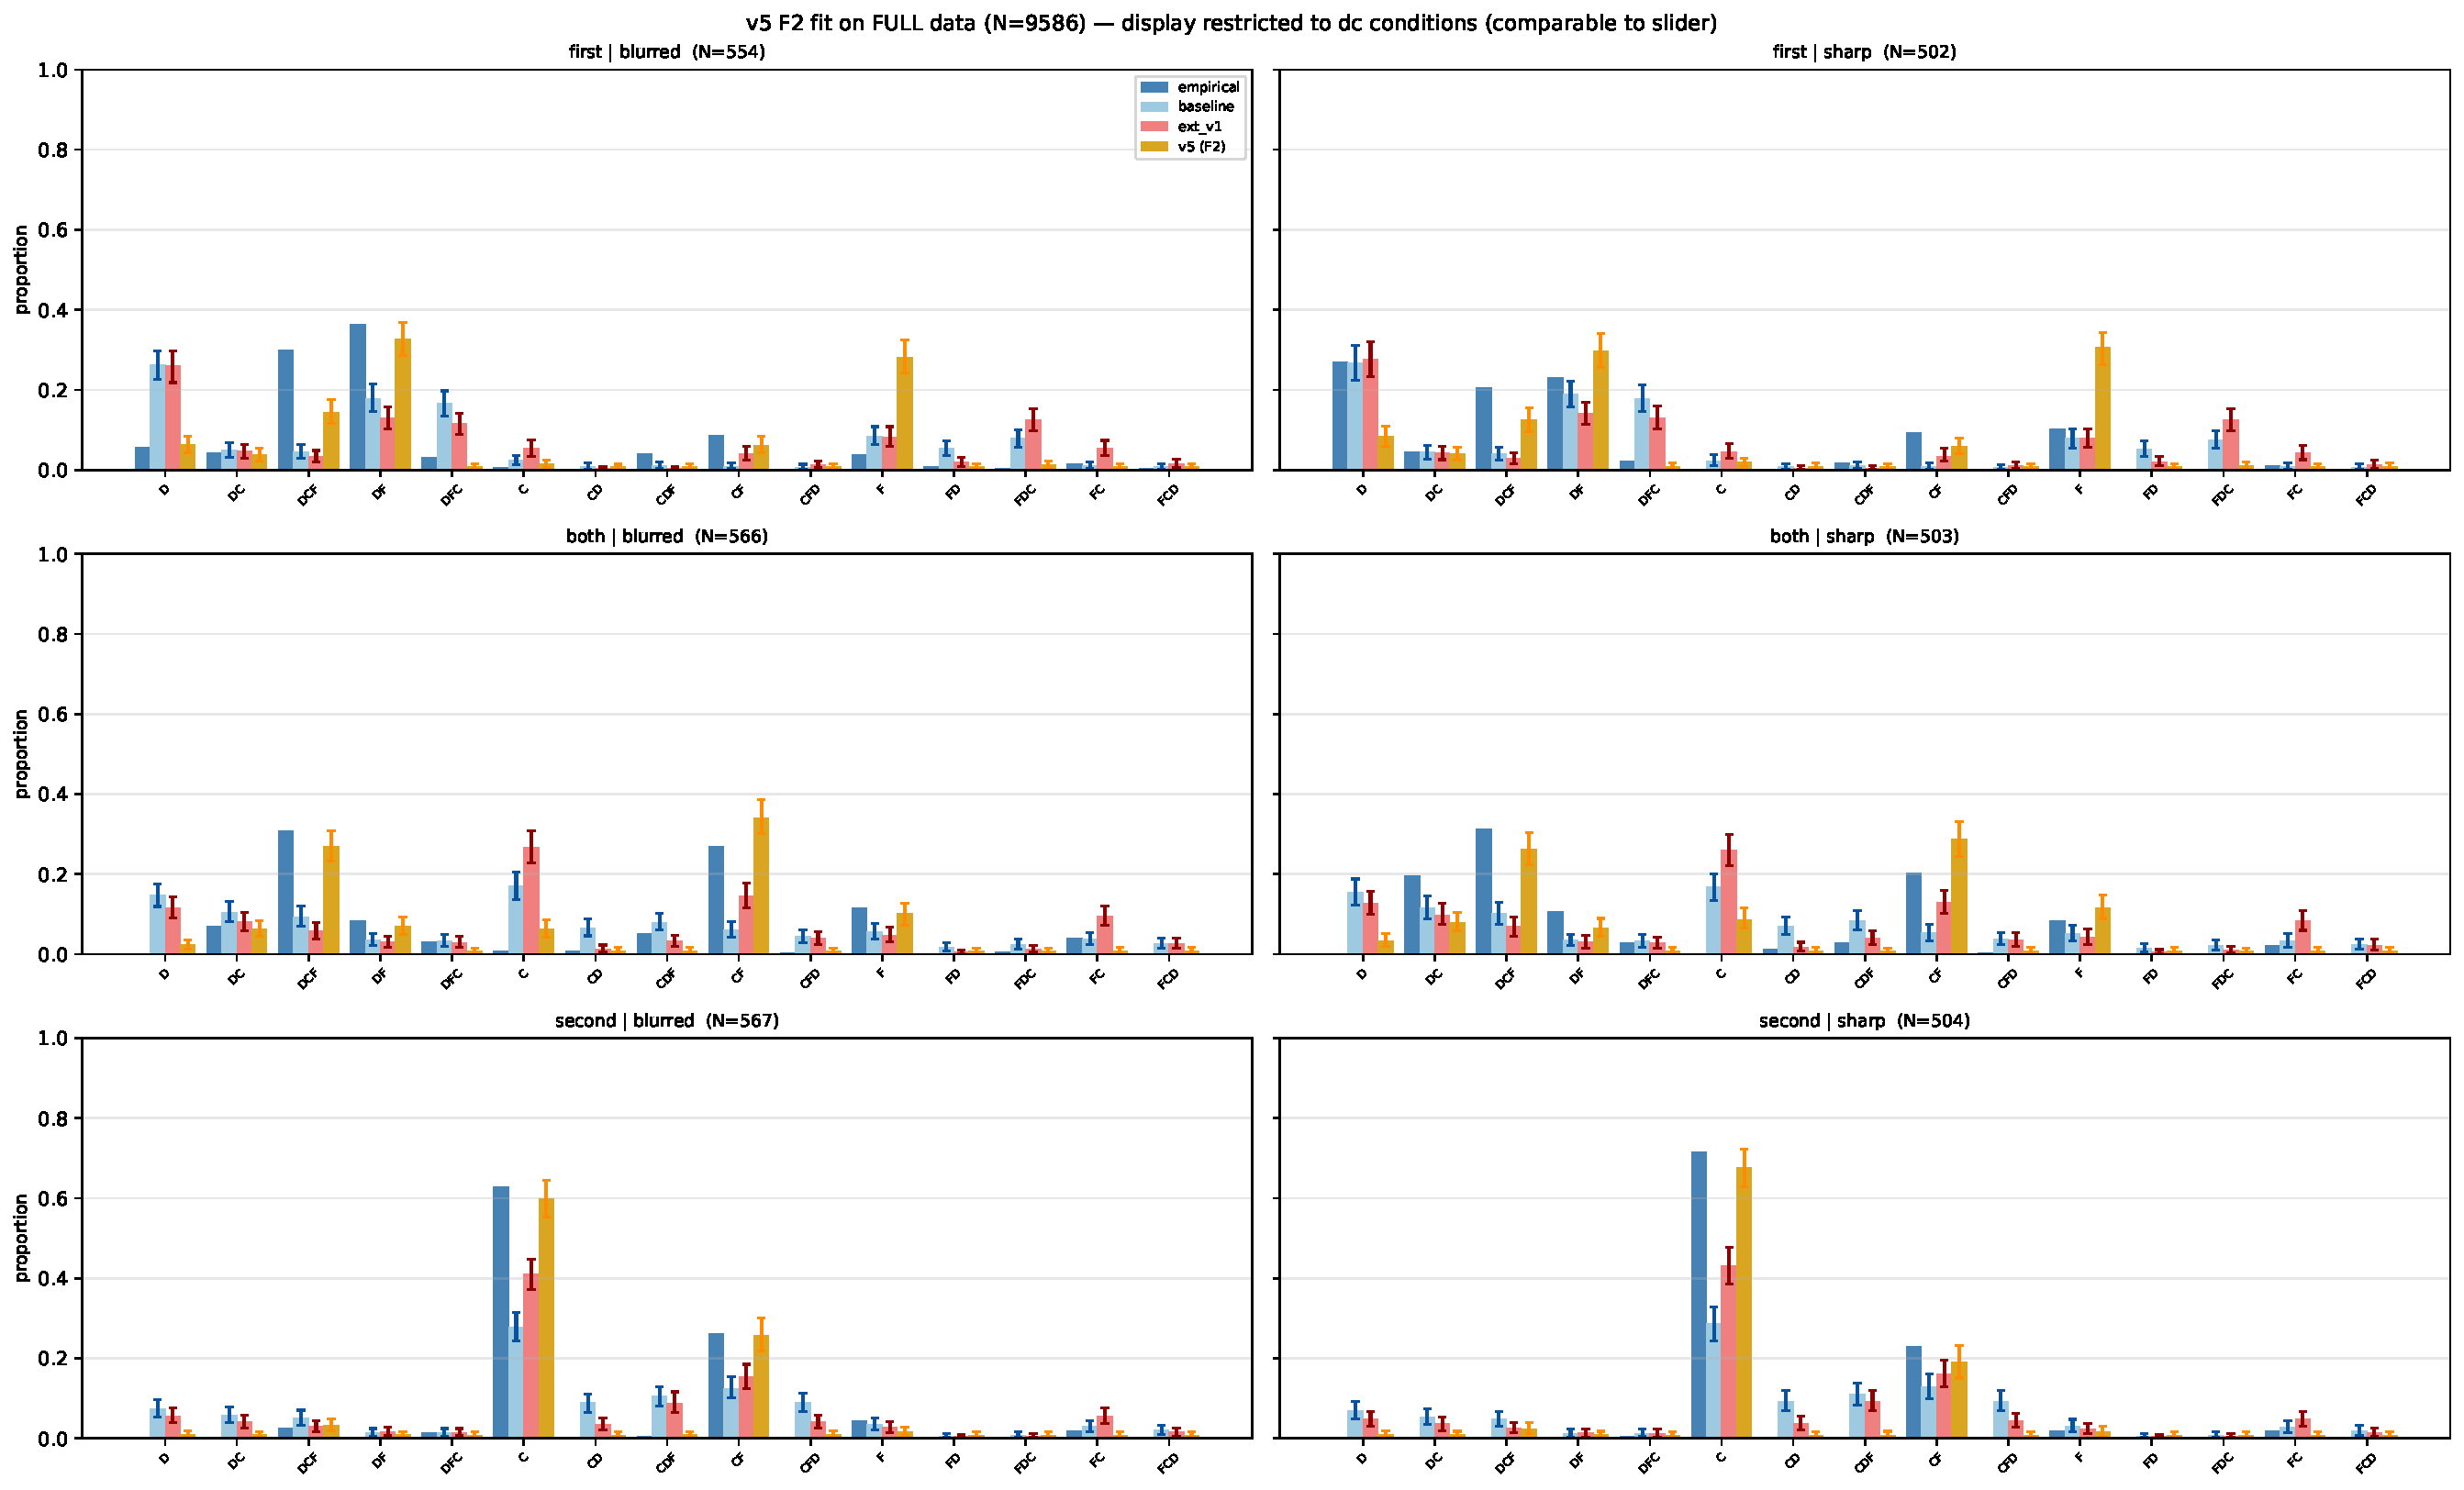
\includegraphics[width=0.98\linewidth]{production_ppc_barplot_v5_fullfit_dc_F2.pdf}
\end{center}
\vspace{-0.3em}
\footnotesize Fit on $N = 9586$ (all 9 conditions); displayed on dc only ($N = 3196$) to remain comparable with the dc-subset slide in the main deck. Rows: \texttt{relevant\_property} (\acct{first} / \accg{both} / \accy{second}). Columns: sharpness. $R^2$ on display $= .84$.
\end{frame}

% ====================================================================
\begin{frame}{Appendix: full-data F2 fit on all 9 conditions}
\vspace{-0.3em}
\begin{center}
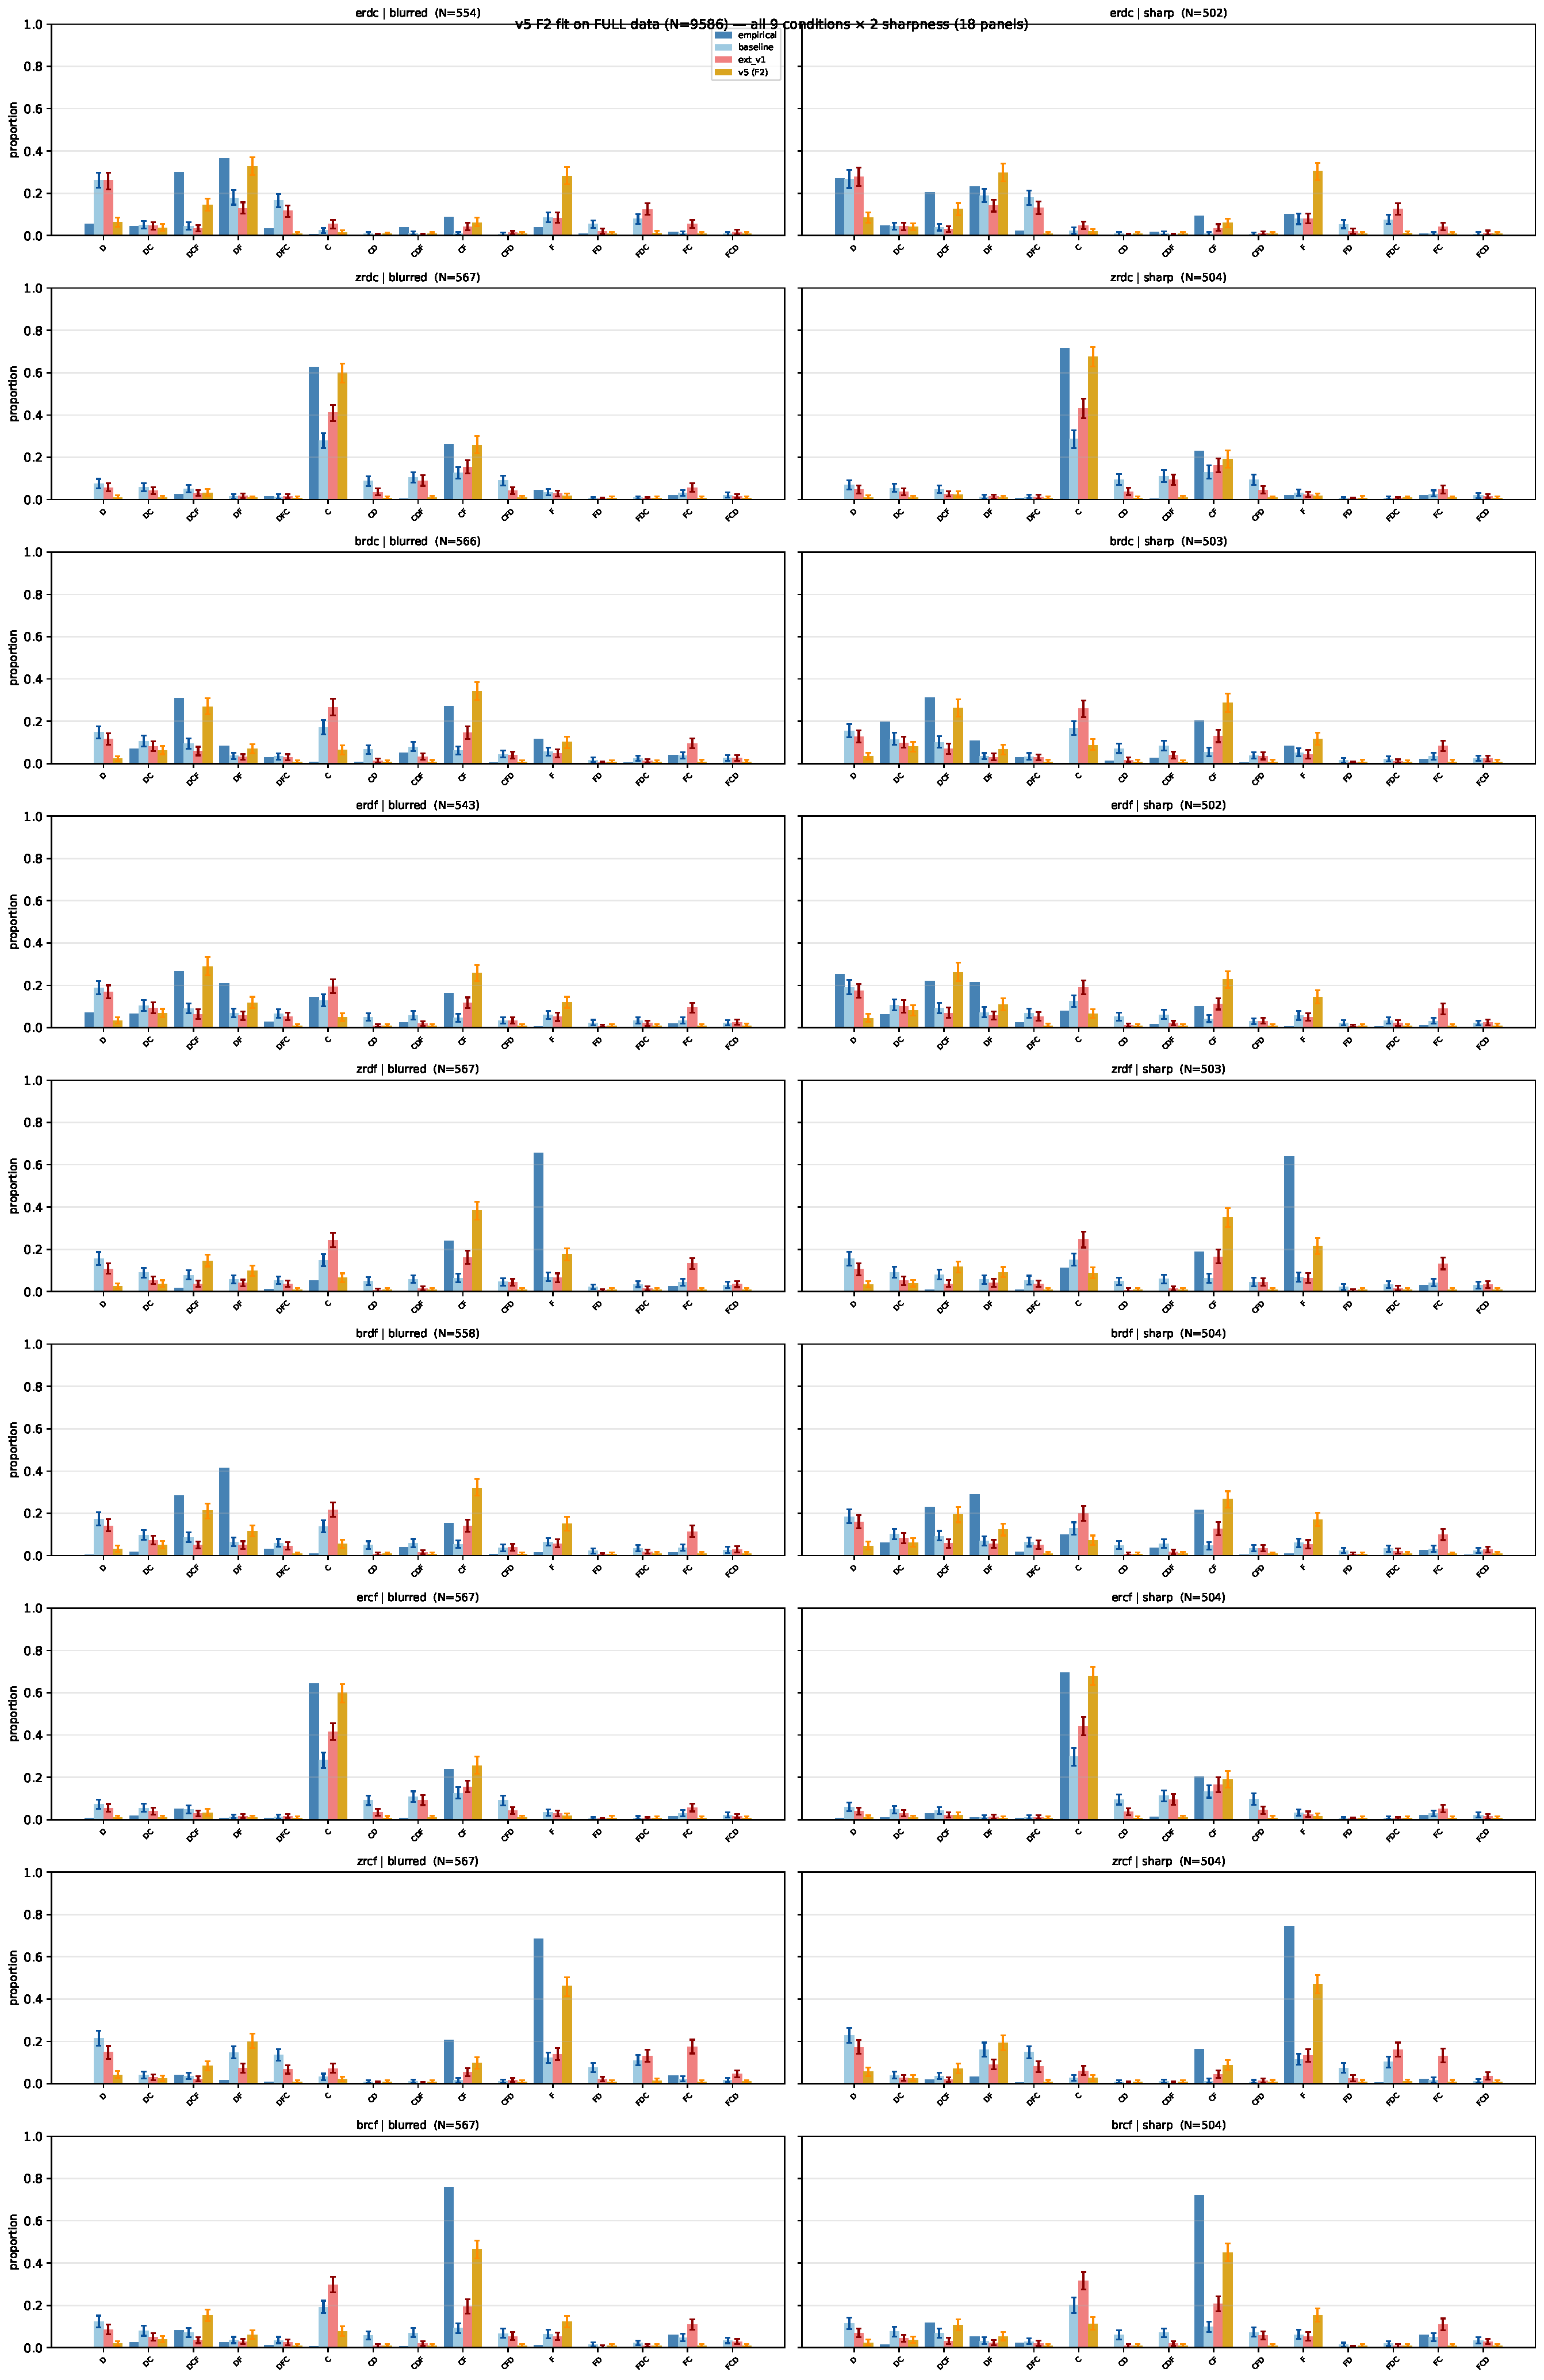
\includegraphics[width=0.92\linewidth]{production_ppc_barplot_v5_fullfit_all9_F2.pdf}
\end{center}
\vspace{-0.3em}
\footnotesize 9 conditions $\times$ 2 sharpness levels $= 18$ panels. v5 F2 (gold) tracks the empirical pattern across the dc, df, and cf families. $R^2$ on display $= .73$ (270 cells); the baseline on the same view is $.10$.
\end{frame}

\end{document}
